\documentclass[a4paper, 10pt]{scrartcl}

\title{MSE Tensor}
\subtitle{Formulary}
\author{dstrebel, s1bischo, sboller, hbaderts, ssteiner}
\date{\today}
\usepackage[T1]{fontenc}
\usepackage[latin1]{inputenc}

% Mathematik-Pakete
\usepackage{amsmath}
\usepackage{amssymb}
\usepackage{amstext}
\usepackage{amsfonts}
\usepackage{mathrsfs}
\usepackage{paralist}
\usepackage[pdftex]{graphicx}
\usepackage{colortbl}
\usepackage[table]{xcolor}
\usepackage{hyperref}
\usepackage{multicol}
\usepackage{tabularx}
\usepackage{booktabs}
\usepackage{siunitx}





%title
\makeatletter         
\def\@maketitle{   % custom maketitle 
	\centering{\LARGE \bf \textsf{\@title}} 
	\smallskip \\
	\centering{\large \bf \textsf{\@subtitle}} 
	\smallskip \\
	\centering{ \bf \textsf {\@author}}
	\medskip \\
	\centering{\bf \textsf{ \@date }}
	\smallskip \\
	\noindent\rule{\textwidth}{0.5pt}
	\smallskip
}
\makeatother


%si units
\sisetup{sticky-per=true,per-mode=symbol}

%header footer
\usepackage[automark]{scrlayer-scrpage}
\pagestyle{scrheadings}
\lohead{\pagemark \hspace{0.3cm }  \textcolor{gray}{\rule{0.25cm}{0.25cm}} \hspace{0.3cm } \leftmark }
\cohead{}
\rohead{}

\rofoot{}
\cofoot{}
\lofoot{}


%geometry
\usepackage[a4paper]{geometry}
\geometry{verbose,tmargin=1.5cm,lmargin=2cm,rmargin=2cm,bmargin=3cm}


\usepackage[english, ngerman]{babel}
\setlength{\parindent}{0cm}
%font
\usepackage{lmodern}

	
	
	
	
	
	




\definecolor{darkgreen}{RGB}{0,100,0}
\definecolor{lightgray}{gray}{0.9}

\renewcommand{\arraystretch}{1.2}

\newcommand{\dx}{\hspace{2pt}dx}
\newcommand{\dd}[1]{\hspace{2pt}d#1}
\newcommand{\laplace}{\Delta}
\newcommand{\qed}{\begin{flushright}
		$\blacksquare \dagger$ \end{flushright}}


\begin{document}
	\maketitle 

	\setlength{\parskip}{0cm}
	\setcounter{tocdepth}{1}	
	
	\tableofcontents 	
	
	\smallskip 
	\rule{\textwidth}{0.5pt}
	\smallskip
	

%%rowcolor



	\section{Description of Physical Phenomena}
	%		\subsection{Einheiten}
{\rowcolors{3}{lightgray}{white}
\renewcommand{\arraystretch}{1.1}	
	\begin{multicols}{2}


		\begin{tabularx}{\linewidth}{lclX}
			\rowcolor{lightblue}\multicolumn{4}{c}{Mathematics}\\			
			$[\nabla]$ &=& \si{1\per\meter} & nabla\\
			$[\laplace]$ &=& \si{1\per\meter\tothe{2}} & laplace\\


			\rowcolor{lightblue}\multicolumn{4}{c}{General}\\
			$[F]$ &=& \si{\newton=\kilogram\meter\per\second\tothe{2}}& Kraft, force \\
			$[E]$ &=& \si{\joule=\kilogram\meter\tothe{2}\per\second\tothe{2}}& Energie, energy \\
			$[P]$ &=& \si{\joule\per\second=\kilogram\meter\tothe{2}\per\second\tothe{3}}& Leistung, power \\
			$[p]$ &=& \si{\pascal= \newton\per\meter\tothe{2}}& Druck, pressure \\
			$[V]$ &=& \si{\meter\tothe{3}}& Volumen, volume\\
			$[T]$ &=& \si{\kelvin}& Temperatur, temperature \\
			$[A]$ &=& \si{\meter\tothe{2}} & Fläche, surface\\



			\rowcolor{lightblue}\multicolumn{4}{c}{Heat}\\
			$[Q_W]$ &=& \si{\joule} & Wärme, heat\\
			$[q_\omega]$ &=& \si{\joule\per\meter\tothe{3}} & Thermische Leitfähigkeit, thermal energy source rate density \\	
			$[W]$ &=& \si{J} & Wärmeenergie, thermal energy\\
			$[\omega]$ &=& \si{\joule\per\meter\tothe{3}} & Energiedichte, thermal energy storage density \\
			$[I_W]$ &=& \si{\joule\per\second=\watt} & Wärmefluss, heat flux\\
			$[j_w]$ &=& \si{\watt\per\square\meter} & Energieflussdichte, thermal energy flux density \\
		\end{tabularx}		
		\begin{tabularx}{\linewidth}{lclX}			
			$[c_p]$ &=& \si{\joule\per\kilogram\kelvin} & spezifischer Wärmekapazität, specific heat capacity\\
			$[\lambda]$ &=& \si{\watt\per\meter\kelvin} & Thermische Leitfähigkeit \\	




			\rowcolor{lightblue}\multicolumn{4}{c}{Mechanics}\\						
			$[m]$ &=& \si{\kilogram} & Masse, mass \\
			$[\rho]$ &=& \si{\kilogram\per\meter\tothe{3}} & Dichte, mass density \\			
			$[p]$ &=& \si{\newton\second} & Impuls \\
			$[J_p]$ &=& \si{\newton} & Impulsfluss, Kraft, Force \\
			$[j_p]$ &=& \si{\newton\per\square\meter} = \si{\pascal} & Impulsflussdichte\\
			$[\sigma]$ &=& \si{\newton\per\square\meter} & Spannung (stress), neg. Impulsflussdichte \\
			$[W]$ &=& \si{\newton\meter} & arbeit, work, mechanical energy\\
			$[\varepsilon l]$ &=& 1& Dehnung (Strain)\\
			$[l_0]$ &=& \si{m} & Ursprüngliche Länge \\
			$[\Delta l]$ &=& \si{m} & Längenausdehnung \\
			$[d]$ &=& \si{\newton\per\meter} & Federkonstant, Spring constant\\
		\end{tabularx}
		
		\begin{tabularx}{\linewidth}{lclX}
			\rowcolor{lightblue}\multicolumn{4}{c}{Particle transport, Stofftransport}\\						
			$[n]$ &=& \si{\mole}& Stoffmenge, Amount of substance\\			
			$[c_n]$ &=& \si{\mole\per\meter\cubed} & particle density concentration\\
			$[I_n]$ &=& \si{\mole\per\second} & particle flux\\
			$[j_n]$ &=& \si{\mole\per\meter\squared\second} & particle flux density\\
			$[D_n]$ &=& \si{\meter\squared\per\second} & Diffusionskoeffizient, diffusion coefficient\\
		\end{tabularx}
			
		\begin{tabularx}{\linewidth}{lclX}
			\rowcolor{lightblue}\multicolumn{4}{c}{Masstransport, Massentransport}\\									
			$[M]$ &=& \si{\kilogram} & masse\\			
			$[I_{M}]$ &=& \si{\kilogram\per\second} & Massenfluss, mass transport, mass flux\\			
			$[j_M]$ &=& \si{\kilogram\per\meter\squared\second} & Massenflussdichte, mass flux density\\
		\end{tabularx}
	\end{multicols}
	

	
	\begin{tabularx}{\linewidth}{lclX}
		\rowcolor{lightblue}\multicolumn{4}{c}{Electricity, Elektrotechnik}\\											
		\multicolumn{4}{c}{\textbf{Electrical network and general Electrodynamics}}\\
		$[U]$ &=& \si{\volt} = \si{\newton\meter\per\ampere\second} & Elektrische Spannung, voltage \\
		$[I]$ &=& \si{\ampere} & Elektrischer Strom, current \\

		$[R]$ &=& \si{\ohm} = \si{\kilogram\square\meter\per\square\ampere\second\tothe{3}} & Elektrischer Widerstand, resistance \\
		$[G]$ &=& \si{\siemens} = \si{\per\ohm} & Elektrische Leitfähigkeit, conductivity \\
		$[C]$ &=& \si{\ampere\second\per\volt} & Capacity, Kapazität \\		
		$[L]$ &=& \si{\henry} & Inductance, Induktivität \\		
		$[\rho]$ &=& \si{\ohm\meter = \kilogram \meter\cubed \per\ampere\tothe{3}\second\tothe{3}} & Spezifischer Widerstand, specific resistance \\
		$[\sigma]$ &=& \si{\per\ohm\meter} = \si{\ampere\per\volt\meter} = \si{\siemens\per\meter} & Spezifische Leitfähigkeit, specific conductivity \\
		$[W]$ &=& \si{\joule} &Electric Energy\\
		$[w]$ &=& \si{\kilogram\per\meter\square\second=\pascal} & electric energy density, Elektrische Energiedichte  \\		
		$[P] = [\dot W]$ &=& \si{\watt} = \si{\joule\per\second} & Elektrische Leistung, power \\

				
				
		%elektrostatik		
		\multicolumn{4}{c}{\textbf{Electrostatics}}\\
		$[Q]=[q]$ &=& \si{\coulomb} = \si{\ampere\second} & Elektrische Ladung, charge \\
		$[\rho]$ &=& \si{\ampere\second\per\meter\cubed} & charge density\\
		$[j]$ &=& \si{\ampere\per\square\meter} & Stromdichte, current density \\	
		$[\vec{E}]$ &=& \si{\volt\per\meter} = \si{\newton\per\coulomb} & Electric Field \\
		$[\varphi]$ &=& \si{\volt} = \si{\kilogram\meter\squared\per\ampere\second\cubed} & Electrostatic potential \\
		$[\vec{p}\:]$ &=& \si{\coulomb\meter} & Electrical dipole moment \\
		$[\Phi]$ &=& \si{\volt\meter} & Electric Flux\\
		$[\vec{D}]$ &=& \si{\coulomb\per\square\meter} & Elektrische Flussdichte, Electric Displacement Field\\
		$[P]$ &=& \si{\coulomb\per\square\meter} & Polarisation Density, Polarisation \\
		$[\chi]$&=& - &Electric susceptibility\\
		$[\varepsilon_0]$ &=& \si{\ampere\second\per\volt\meter} = \si{\square\coulomb\per\newton\square\meter} & permittivity of free space, Elektrische Feldkonstante \\

		$[w_E]$ &=& \si{\watt\second\per\meter\cubed} = \si{\joule\per\meter\cubed} & energy density\\
		$[k]$ &=& \si{\volt\meter\per\ampere\second} & Coulomb-constant \\				
		%electro magnetostatics
		\multicolumn{4}{c}{\textbf{Magnetostatics}}\\
	
		$[B]$ &=& \si{\tesla} (Tesla) = \si{\kilogram\per\ampere\square\second} = \si{\newton\per\ampere\meter} = \si{\volt\second\per\square\meter} & Magnetic flux density, Magnetische Flussdichte \\
		$[H]$ &=& \si{\ampere\per\meter} & Magnetic field strength, Magnetische Feldstärke \\
		

		$[\mu_0]$ &=& \si{\volt\second\per\ampere\meter} & permeability of free space, Magnetische Feldkonstante \\
		$[\bm m]$ &=& \si{\ampere\meter\squared} & magnetic moment, Magnetisches Moment\\
	\end{tabularx}

	\subsection{constants}
	\begin{tabularx}{\linewidth}{lcX}
		1 \si{\mol} = $N_A$  &=& $6.022\cdot 10^{23}$\\
		$\mu_0$ &=& $4\pi\cdot10^{-7} \si{\volt\second\per\ampere\meter}$\\
		$\epsilon_0$ &=& $8.854\cdot10^{-12} \si{\ampere\second\per\volt\meter}$\\
		$k = 1/(4\pi\epsilon_0)$ &$\approx$& $8.988\cdot 10^9 \quad Nm^2C^{-2}$ \\
		$c$ &=& $3\cdot 10^8 \si{\meter\per\second}$\\
	\end{tabularx}
	
}%rowcolor	tabularx		
	%	\renewcommand{\arraystretch}{2}	
{\rowcolors{3}{lightgray}{white}
	\subsection{Begriffe}
	\begin{multicols}{2}
		
	\begin{tabularx}{\linewidth}{lX}
		\multicolumn{2}{c}{\textbf{Classes of Physical Laws}}\\
		Basic laws, balance equation & \\
		Material laws, consecutive laws & \\
		 
		\multicolumn{2}{c}{\textbf{Uniform (homogeneous) Systems}}\\
		spatially constant& \\		
		intensive quantities& pressure, temperature\\		
		extensive quantities & substance like, impulse, volume\\
	\end{tabularx}
	\vfill\columnbreak
		\begin{tabularx}{\linewidth}{lX}
			\multicolumn{2}{c}{\textbf{Balance equation}}\\
			$\dfrac{dG}{dt} = \sum\limits_{i} I_{i} + Q$ & $ G, I, Q$ : extensive \\
			\multicolumn{2}{c}{
				$\dfrac{dG}{dt}$: change rate $\quad$
				$I$: flux $\quad$
				$Q$: sourceterm} \\		
			substance & substace density $ \Rightarrow 1/m^3$\\
			flux & flux density $  \Rightarrow 1/m^2$\\
			source & source density $  \Rightarrow 1/m^3$\\
			\multicolumn{2}{c}{\textbf{material properties}}\\
			iostropic & independent of spatial direction\\
			homogeneous & spatially constant\\
			linear & balance equation always, consecutive not\\
		\end{tabularx}
	\end{multicols}
\renewcommand{\arraystretch}{1.2}			
	
	\subsection{Balance equation, Bilanzgleichungen}
	{
		\begin{tabularx}{\linewidth}{XXXll}
			\hline
			& Stoffliche Grösse & Potential & \multicolumn{2}{c}{Balance Equation} \\
			& & & uniform & distributed, local \\ \hline
			Charge Transport & Charge $Q$ & El. Potential $\Phi$ & $\frac{dQ}{dt}=I_Q$ & $ \frac{\partial p_Q}{\partial t}=-\nabla\cdot j_Q$ \\ \hline
			Heat Transport & Thermal energy \newline $W$ & Temperatur $T$ & $\frac{\partial W}{\partial t}= I_W+Q_W$ & $\frac{\partial w}{\partial t}= -\nabla \cdot j_W+q_W$  \\ \hline
			Particle Transport & Partical number \newline $N$ & Particle density \newline $c$ & $\frac{dN}{dt}=I_N+Q_N$ & $\frac{dp}{dt}=-\nabla \cdot j_W +q_W$ \\ \hline
			Mechanics (Momentum Transport) & Momentum $p$ & Velocity $v$  & $\frac{\partial p}{\partial t}=F$ &  $\frac{\partial \sigma_{ik}}{\partial x_k} + \rho g_i$ = 0\\ 
			\hline
		\end{tabularx} }
		
		\subsection{Constitutive Laws}
		\begin{tabularx}{\linewidth}{Xp{3cm}p{4.55cm}X}
			\hline
			& Storage Laws & Flux Laws & Source Rates and Sourcerate Densities \\ \hline
			Charge Transport & charge carrier diffusion equation & $j_Q=-\sigma \cdot \nabla\varphi \equiv \sigma \cdot E$ \newline (Microscop. Ohmic law) & $q_+ = - q_-$ \\
			Heat Transport & $w=c_p \rho T$ & $j_W=-\lambda \cdot \nabla T$  (Fourier's law)& $Q_W = -(\phi_2-\phi_1)I_Q$\newline $q_W = -\nabla\Phi\cdot j_Q$  \\ 
			Particle Transport (Diffusion) & c=c & $j_N=- D \cdot \nabla c_N$ &  \\ 
			Mechanics & uniform: $p=mv$,\newline local : $\pi=\rho v$ & $F_{hook} = - k \Delta u$ (Hook's Law)\newline $F_{visc}=-C \eta \cdot v$ (Viscous Drag) & $F_{grav} = M g$\newline $f_{grav}=\rho g$ \\ 
			\hline
		\end{tabularx} 
}%rowcolor	tabularx				

	
	\section{Vector Analysis and Integral theorems}
	%	
		\subsection{General Remarks}		
		\textcolor{blue}{\textbf{Gradient}}: 

		\textbf{Direction, Angle}: points to the steepest ascent.
		
		\textbf{Absolute Value}: is the greater, the stronger a value changes at a position.
		
		\textbf{scalar field}$\Rightarrow$ \textbf{vector field}
				
		\textcolor{blue}{\textbf{Divergence}}:
		
		Gives the tendencie of a vector field, to flow away from a point.
		
		$\operatorname{div}\vec F(\vec r) = q(\vec r) \begin{cases}
			> 0, & \text{source, quelle}\\
			= 0, & \text{source free}\\
			< 0, & \text{sink, senke}
		\end{cases}$
		
		\textbf{Vector field} $\Rightarrow$ \textbf{scalare field}
		
		\textcolor{blue}{\textbf{Curl, Rotation}}
		
		Tendency to rotate around a point. 
		
		The rotation of a vector field is a vector field of pseudo vectors. 
		
		Describes the local curl density of a vector field.		
		
		\textbf{vector field}$\Rightarrow$ \textbf{vector field}

		\textcolor{blue}{\textbf{signs and notation}}: 
		
		\begin{tabularx}{\linewidth}{l|X}
		$\text{Nabla operator:}\quad \nabla \: \mathrm{oder} \: \vec \nabla = \left (\dfrac\partial{\partial
			x_1},\ldots, \dfrac\partial{\partial x_n}\right) $ 
		&
		$\text{Laplace operator:}\quad \laplace \: \mathrm{oder} \: \vec \laplace = \left (\frac{\partial^2}{\partial
			x_1^2},\ldots, \frac{\partial^2}{\partial x_n^2}\right)$
		\\
		\hline
		$\text{Scalar function:}\quad f = f(x,y,z)$
		&
		$\text{vector field:}	\quad \vec F = \begin{pmatrix} F_1 \\ F_2 \\ F_3 \end{pmatrix}$
		\\
		\hline
		\multicolumn{2}{l}{
		$
		\text{Vector product in cartesian coordinates:}\quad\vec{a}\times\vec{b} = \begin{vmatrix}
		\textbf{i} & \textbf{j} & \textbf{k} \\ a_1 & a_2 & a_3 \\ b_1 & b_2 & b_3\\ \end{vmatrix} =
		\begin{pmatrix}a_1 \\ a_2 \\ a_3\end{pmatrix} \times
		\begin{pmatrix}b_1 \\ b_2 \\ b_3 \end{pmatrix} = \begin{pmatrix} a_2b_3 - a_3b_2
		\\ a_3b_1 - a_1b_3 \\ a_1b_2 - a_2b_1 \end{pmatrix}$}\\
	\hline 
	\end{tabularx}
			
\renewcommand{\arraystretch}{2}		
		\begin{tabularx}{\linewidth}{lllllX}
			\hline
			Function & &Nabla & &Differential form & Note \\
			\hline
			$\operatorname{grad}(f)$ &=& 
			$\nabla f$ &=&
			 $ 
			\begin{pmatrix} \dfrac{\partial f}{\partial x}, \quad\dfrac{\partial f}{\partial
				y}, \quad \dfrac{\partial f}{\partial z} \end{pmatrix}^T$&\\	
			\hline 
			$\operatorname{div}\vec F$ &=& 
			$\nabla \cdot \vec F$&=&
			$\dfrac{\partial}{\partial x_1}F_1 + \dfrac{\partial}{\partial x_2}F_2+ \dfrac{\partial}{\partial x_3}F_3$&
			$\operatorname{div}\vec F = \dfrac{\sum_i I_i}{V}$\\
			\hline
			$\mathbf{\operatorname{rot}}\,\vec F$ &=& 
			$\nabla\times \vec F$ &=& 
			$\begin{pmatrix} \dfrac{\partial}{\partial x} \\ \dfrac{\partial}{\partial y} \\
				\dfrac{\partial}{\partial z} \end{pmatrix} \times \begin{pmatrix} F_x\\ F_y\\ F_z
			\end{pmatrix} = \begin{pmatrix} \dfrac{\partial F_z}{\partial y} - \dfrac{\partial
				F_y}{\partial z} \\ \dfrac{\partial F_x}{\partial z} - \dfrac{\partial
				F_z}{\partial x} \\ \dfrac{\partial F_y}{\partial x} - \dfrac{\partial
				F_x}{\partial y} \end{pmatrix}$&
			$\mathbf{\wedge = \times} \newline$\\ 
			&&
			&=&
			$ \left (\dfrac{\partial F_y}{\partial x} - \dfrac{\partial F_x}{\partial y}\right )\vec e_z$ & 2 Dimensional\\
			\hline
		\end{tabularx}

\renewcommand{\arraystretch}{1}				


	
	\subsection{Calculation rules (Bronstein p.731)}
	
{\rowcolors{3}{lightgray}{white}	
\renewcommand{\arraystretch}{1.2}					
	\begin{tabularx}{\textwidth}{|X|X|}
		\hline 
		\multicolumn{2}{|l|}{
		Vector filds : $\vec F$, $\vec G$  $\qquad$ 
		Scalar fields: $U$, $V$	           $\qquad$ 
		constant, constant field: $c, \vec{c}$}\\			
		
		\hline
		$\operatorname{grad}\,c=\vec{0}$ & $\operatorname{grad}\,(c\cdot u)=c\cdot\operatorname{grad}\,U$    \\

		$\operatorname{grad}\,(U+V)=\operatorname{grad}\,U+\operatorname{grad}\,V$ &
		$\operatorname{grad}\,(U\,V) = U\ \operatorname{grad}\,V + V\ \operatorname{grad}\,U$\\

		$\label{eqn:ProduktregelEinesGradientMitPotenzen}
		\operatorname{grad}\,(U^n) = n\, U^{n-1}\ \operatorname{grad}\,U \text{ für } n\neq 0$&
		$\operatorname{rot}(\operatorname{grad}U)=\nabla \times (\nabla U) = 0$ \\
		\hline\hline
		$\operatorname{div}\,\vec{c}=\vec{0}$&
		$\operatorname{div}\,(c\cdot \vec{F})=c\cdot\operatorname{div}\,\vec{F}$ \\
		
		$\operatorname{div}\,(\vec{F}+\vec{G})=\operatorname{div}\,\vec{F}+\operatorname{div}\,\vec{G}$ &
		$\operatorname{div}\,(U\,\vec{F}) = U\ \operatorname{div}\,\vec{F} + \vec{F}\cdot \operatorname{grad}\,U$\\		

		$\operatorname{div}\,(\vec{F} \times\vec{G})=\vec{G}\cdot \operatorname{rot}\,\vec{F} - \vec{F}\operatorname{rot}\,\vec{G}$ &
		$\operatorname{div}(\operatorname{rot}\vec{F}) = \nabla \cdot (\nabla \times\vec F) = 0$\\
		\hline\hline
		
		$\operatorname{rot}\,(\vec{F}+\vec{G})=\operatorname{rot}\,\vec{F}+\operatorname{rot}\,\vec{G}$ &
		$\operatorname{rot}\,(c \vec{F})=c\operatorname{rot}\,\vec{F}$ \\

		$\operatorname{rot}\,(U\,\vec{F}) = U\ \operatorname{rot}\,\vec{F} + \operatorname{grad}\,U \times \vec{F}$&
		$\operatorname{rot}\,(\vec{F} \times\vec{G}) =\newline (\vec{G}\cdot \operatorname{grad})\,\vec{F} - (\vec{F}\cdot \operatorname{grad})\,\vec{G} + \vec{F}\operatorname{div}\vec{G} - \vec{G}\operatorname{div}\,\vec{F}$
		\\
		\hline\hline
		$	\operatorname{rot}(\operatorname{rot}\vec{F}) = \operatorname{grad}(\operatorname{div}\vec{F}) -\Delta \vec{F}$&\\

		$\operatorname{grad}(UV)=U\operatorname{grad}V+V\operatorname{grad}U $ &
		$\operatorname{grad}(\vec{F}\cdot \vec{G}) = (\operatorname{grad}\vec{F})^{\operatorname t}\vec{G} + (\operatorname{grad}\vec{G})^{\operatorname t}\vec{F} $ \\

		$	\operatorname{div}(U\vec{F})=U\operatorname{div}\vec{F}+\vec{F}\cdot\operatorname{grad}U $&
		$\operatorname{div}(\vec{F}\times \vec{G})= \vec{G} \cdot\operatorname{rot}\vec{F} -\vec{F}\cdot\operatorname{rot}\vec{G} $ \\				

		$\operatorname{rot}(U\vec{F})= U\operatorname{rot}\vec{F}-\vec{F}\times\operatorname{grad}U\ $& 
		$\operatorname{grad}\,\varphi(U) = \dfrac{d\varphi}{dU}\operatorname{grad}\,U$
		\\
		\hline
	
		
	\end{tabularx}
}
\renewcommand{\arraystretch}{1.2}		

	\paragraph{Potential Field}
		If a vector field is path independant it is called conservative. This vector field is the gradient of a potential function $\phi$
		
		\begin{multicols}{3}
			$$ -\int\limits_a^b \vec F\cdot d\vec x = \phi(\vec b) - \phi(\vec a) $$ \vfill\columnbreak
			$$ \oint \vec F\cdot d\vec x = 0 $$ 
			$$ \nabla \times \vec F = 0  $$ \vfill\columnbreak
			$$ F = \operatorname{grad}\phi $$
		\end{multicols}
		
		
	\paragraph{Line integral}~\\
	\begin{tabularx}{\columnwidth}{lp{2.5cm}p{4cm}X}
	\hline 
		\multicolumn{4}{c}{receipt to Line integrals in a vector field}\\
	\hline 
		1& Partition & Divide the curve into pieces & $I = \int\limits_C\bm fd\bm r = \int\limits_{C_1}\bm fd\bm r_1 + \int\limits_{C_2}\bm fd\bm r_2+\dots = \sum\limits_i \int\limits_{C_i}\bm fd\bm r_i$\\
		2& Line vector& 
		 Describe the curve $C_i$ as a function of t & $\bm r_i(t) = \left(x_i(t), y_i(t), z_i(t)\right)^T\quad t\in[a,b]$\\
		3& Derivative & take the derivative of $\bm r_i(t)$ & $\bm r_i'(t) = \left(x_i'(t), y_i'(t), z_i'(t)\right)^T \quad d\bm r_i = \bm r_i'(t) dt $\\
		4& parametrize the field  & put $\bm r_i(t)$ into the vector field function & $\bm f(x,y,z) = \bm f(\bm r_i(t) ) = \bm f(x_i(t), y_i(t), z_i(t))$\\
		5& integrals & calculate the integrals & $I_i = \int\limits_{C_i} = \bm f(\bm r_i(t))\cdot \bm r_i'(t)dt$\\
		6& sum up & summarize the pieces & $I = \sum\limits_i I_i$\\
		\hline 
	\end{tabularx}
	scalar field $$I = \int\limits_C f d \bm r = \int\limits_{a}^b f(\bm r(t))\; |\bm r'(t)| dt$$
	
	vector field $$I = \int\limits_C \bm f d\bm r = \int\limits_{a}^b \bm f(\bm r(t))\; \cdot \bm r'(t) dt$$
		
	\paragraph{special vectors}  
	$\bm r = \begin{pmatrix} x\\y\\z\end{pmatrix} \qquad |\bm r| = r = \dfrac{1}{\sqrt{x^2+y^2+z^2}}$
	
	$\nabla\left(\dfrac{1}{r}\right) = -\dfrac{\bm r}{r^3}\qquad
	\nabla\left(\dfrac{1}{r^2}\right) = -\dfrac{2\bm r}{r^4}\qquad
	\nabla\left(\dfrac{1}{r^3}\right) = -\dfrac{3\bm r}{r^5}\qquad
	\nabla (\bm r \bm F) = \bm F$

	\subsection{Integral theorems}
	
		
		\textcolor{blue}{\textbf{Divergence Theorem of Gauss}}: Volume integral: Divergence of a Vectorfield $\Rightarrow$ Surface integral: Vectorfield\\
		
		$$\int_V \operatorname{div} \vec{F} \; \mathrm dV = 
				\int_V \nabla\cdot \vec{F} \; \mathrm dV =
				\oint_{S} \vec F \cdot\vec n\; \mathrm dA
		$$

	\textcolor{blue}{\textbf{Stoke's Theorem}}: Surface integral: rotation of a vector field $\Rightarrow$ line integral along the surface: vector field  
	
	$$\int_{F} \operatorname{rot} \vec F \cdot d \vec A =
		\int_{F} \nabla \times \vec F \cdot d \vec A =
		\oint_{\partial F} \vec F \cdot d \vec r $$
	


	


	\section{Mathematical Basics of Tensors}
	%	\subsection{Basics}
		All tensor rules are only valid in cartesian coordinate systems
		
		\begin{tabularx}{\columnwidth}{lX}
			\multicolumn{2}{c}{\textbf{Einsteins notation}}\\
			$w_i=\sum\limits_{j=1}^{3}A_{ij}v_j=A_{ij}v_j$ &	Whenever a \textbf{repeated} index appears on one side of a formula, a summation is silently implied!\\			
			\textbf{Vector definition}& Vectors are physical quantities whose  coefficients transform under rotations of the coordinate system\\
			\textbf{Rank of a tensor} & The rank of a tensor is given through the number of its indices\\
			\textbf{Delta tensor} & $\delta_{ij} = \begin{cases} 0 & i\neq j\\ 1 & i = j \end{cases}$\\
			\textbf{Orthogonal matrices} & $R^{-1} = R^T \quad RR^t = E \quad R^TR=E \qquad \sum\limits_{i=1}^3 d_{ji}d_{ki} = \delta_{kj} \qquad \sum\limits_{i=1}^3 d_{ik}d_{ij} = \delta_{ij}$\\
			\textbf{notes to eigenvalues} & the trace is the sum of the eigenvalues: $\operatorname{tr}\mathbf{A} = \sum \operatorname{eig}\mathbf{A}$ \newline 
			                                the determinant is the product of the eigenvalues: $\operatorname{det}\mathbf{A} = \prod \operatorname{eig}\mathbf{A}$  \\
		\end{tabularx}
	


	\subsection{Special Tensor}
	\paragraph{2nd Rank} Tensor of 2nd rank behave like matrices. Every Tensor can be divided into a symmetric and an antisimmetric part.
			$$\mathbf{T}=\mathbf{T}^{sym}+\mathbf{T}^{asym} = \frac{1}{2}\left(\mathbf{T}+\mathbf{T}^T\right) + \frac{1}{2}\left(\mathbf{T}-\mathbf{T}^T\right)$$
			
			$$	\mathbf{T}^{sym}=\frac{1}{2}\left(\mathbf{T}+\mathbf{T}^T\right) \qquad t_{ij} = t_{ji}$$
			$$	\mathbf{T}^{asym}=\frac{1}{2}\left(\mathbf{T}-\mathbf{T}^T\right) \qquad t_{ij} = -t_{ji} \qquad t_{11} = t_{22} = t_{33} = 0$$

		A Symetric 2nd order tensor can be brought into a System of Principal Axis. Eigenvalues can be calculated with the well known formula: $|\mathbf{T}-\lambda \mathbf{I}| = 0$
		
		$$ \mathbf{T}^{sym} = \mathbf{R}^T \mathbf{T} \mathbf{R} \qquad \mathbf{R}\text{: columns are Eigenvectors of \textbf{T}}$$ 		
		
		$$ \mathbf{T}^{sym} = \begin{pmatrix}
		t_{11} & 0 & 0 \\ 0 & t_{22} & 0 \\ 0 & 0 & t_{33} \\
		\end{pmatrix}$$

		
		
	\paragraph{Invariant tensors} Invariant tensors have the same components in every coordinate systems. Transformation doesn't change the Invariant tensor.
	
	\begin{tabularx}{\columnwidth}{lXX}
		\hline
		2nd rank unit tensor & $I_{ij} = \delta_{ij}$ &\\
		trace of 2nd rank & $\operatorname{tr} \mathbf{E} = E_{ii} = \sum\limits_{i=1}^3 E_{ii}$ &\\
		4th rank unit tensor & $\mathbb{I} = I_{ijkl} = \frac{1}{2}(\delta_{ik}\delta_{jl} + \delta_{il}\delta_{jk}) $ & both of the 4th rank tensors are isotropic\\
						 & $\mathbb{E} = E_{ijkl} =  \delta_{ij}\delta_{kl}$ &\\
						 
		$ \mathbb{I}^{eng}=
		\begin{pmatrix}
			1 & 0 & 0 & 0 & 0 & 0 \\ 
			0 & 1 & 0 & 0 & 0 & 0 \\ 
			0 & 0 & 1 & 0 & 0 & 0 \\ 
			0 & 0 & 0 & \frac{1}{2} & 0 & 0 \\ 
			0 & 0 & 0 & 0 & \frac{1}{2} & 0 \\ 
			0 & 0 & 0 & 0 & 0 & \frac{1}{2}
		\end{pmatrix}$& 
		
		$
		\mathbb{E}^{eng}=
		\begin{pmatrix}
		1 & 1 & 1 & 0 & 0 & 0 \\ 
		1 & 1 & 1 & 0 & 0 & 0 \\ 
		1 & 1 & 1 & 0 & 0 & 0 \\ 
		0 & 0 & 0 & 0 & 0 & 0 \\ 
		0 & 0 & 0 & 0 & 0 & 0 \\ 
		0 & 0 & 0 & 0 & 0 & 0
		\end{pmatrix} 
		$	&
		$ \mathbb{I_{\text{bischsil}}}^{eng}=
		\begin{pmatrix}
		1 & 0 & 0 & 0 & 0 & 0 \\ 
		0 & 1 & 0 & 0 & 0 & 0 \\ 
		0 & 0 & 1 & 0 & 0 & 0 \\ 
		0 & 0 & 0 & 1 & 0 & 0 \\ 
		0 & 0 & 0 & 0 & 1 & 0 \\ 
		0 & 0 & 0 & 0 & 0 & 1
		\end{pmatrix}$
			\\
							 
   	   \hline
	\end{tabularx}
	
	\subsection{Transformations and changes of coordinate systems}
	
	\begin{tabularx}{\columnwidth}{p{4.8cm}Xp{4.8cm}}	
		\hline 
		\multicolumn{2}{p{8cm}}{\textbf{Passive rotation}: rotation of the coordinate system (basis vectors)} & \textbf{Active rotation}: rotation of the vector  \\
		\hline
		1st rank (vector) & Tensor notation: $v_j' = R_{ji}v_i$  \newline matrix notation: $v' =  \textbf{R}v$ & $v_i$: vector (could be basis $e_i$)\newline $R$: orthogonal transformation matrix\\
		\hline 
		2nd rank (matrice) & Tensor notation: $M_{ij}' = R_{im}R_{jn}M_{mn}$  \newline matrix notation: $M' =  \textbf{R}M\textbf{R}^T$ & $M_{ij}$: 2nd rank tensor \newline $R$: orthogonal transformation matrix\\
		\hline 
		higher rank & $F_{ijkl}' = R_{im}R_{jn}R_{ko}R_{lp}F_{mnop}$  \newline & $F_{ijkl}$: 4th rank tensor \newline $R$: orthogonal transformation matrix\\					
		\hline
					
		$R_x(\alpha) = \begin{pmatrix} 
		1 &   0         & 0           \\
		0 & \cos \alpha & -\sin \alpha \\
		0 & \sin \alpha &  \cos \alpha
		\end{pmatrix} $ &
		$R_y(\alpha) = \begin{pmatrix} 
		\cos \alpha  & 0 & \sin \alpha \\
		0         & 1 &  0          \\
		-\sin \alpha & 0 & \cos \alpha
		\end{pmatrix} $ &
		$R_z(\alpha) = \begin{pmatrix} 
		\cos \alpha & -\sin \alpha & 0 \\
		\sin \alpha &  \cos \alpha & 0 \\            
		0        &  0           & 1
		\end{pmatrix}$\\
					
	\hline 
	\end{tabularx}
	

	\subsection{Tensor Algebra}
	\begin{tabularx}{\columnwidth}{p{3cm}lXX}
		\hline 
		Operator & General & Tensor algebra & notes\\ 
		\hline 
		Addition & $C=A+B$ & $C_{ij}=A_{ij}+B_{ij}$  & valid for each rank\\ 
		
		Multiplication with a scalare& $B=\alpha A$ & $B_{ij}=\alpha A_{ij}$ & valid for each rank\\ 
		
		Tensor multiplication &  $C=AB$ & $C_{ij}=A_{ik}B_{kj}$ & 2nd $\cdot$ 2nd = 2nd rank\newline corresponds to matrix-matrix multiplication\\
		 &$w=Av$ & $w_i=A_{ij}v_{j}$ & 2nd $\cdot$ 1st = 1st rank\newline corresponds to matrix-vector multiplication \\
		
		Dyadic product & $\textbf{M} = a \otimes b $ & $M_{ij} = a_i b_j$  & forming 2nd rank tensor\\ 
				  	   & $\mathbb{C} = A \otimes B $ & $C_{ijkl} = A_{ij} B_{kl}$ & forming 4th rank tensor\\
		 
		Gradient    & $g = \nabla T$ & $g_i = \dfrac{\partial T}{\partial x_i} $ & \\
		
		Contraction\newline Tensorverjüngung &  $c=ab = a:b$ & $c=a_{i}B_{i}$ & 1nd : 1nd = 0th rank  \\
									  		 &  $c=A:B$ & $c=A_{ij}B_{ij}$ & 2nd : 2nd = 1st rank \\
											 & $B=\mathbb{D}:A$ & $B_{kl}=D_{klij}A_{ij}$  & 4th : 2nd = 2nd rank\\

		Transposition & $\mathbf{A}^T$ & $A^T_{ij} = A_{ij}$ & only for second rank\\
		\hline 
	\end{tabularx} 


	\subsection{Engineering notation}
	Engineering notation for special tensors of 2nd rank
	$$ \mathbb{I}^{eng}=(1,1,1,0,0,0) $$
	$$\sigma^{eng} = (\sigma_{11},\sigma_{22},\sigma_{33},\sigma_{23},\sigma_{13},\sigma_{12} )^T$$
	
	$$\epsilon^{eng} = (\epsilon_{11},\epsilon_{22},\epsilon_{33},2\epsilon_{23},2\epsilon_{13},2\epsilon_{12} )^T$$	
	
	A symmetric tensor of 4th rank can be written as $C_{ijkl} = C_{jikl} = C_{ijlk} = C_{klij} $
	
	$$\mathbb{C}^{eng}= \begin{pmatrix}
			C_{11}&C_{12}&C_{13}&C_{14}&C_{15}&C_{16}\\
			C_{21}&C_{22}&C_{23}&C_{24}&C_{25}&C_{26}\\
			C_{31}&C_{32}&C_{33}&C_{34}&C_{35}&C_{36}\\
			C_{41}&C_{42}&C_{43}&C_{44}&C_{45}&C_{46}\\
			C_{51}&C_{52}&C_{53}&C_{54}&C_{55}&C_{56}\\
			C_{61}&C_{62}&C_{63}&C_{64}&C_{65}&C_{66}
		\end{pmatrix}$$
	
		$$\begin{pmatrix}
			1&2&3&4&5&6\\
			\updownarrow&\updownarrow&\updownarrow&\updownarrow&\updownarrow&\updownarrow\\
			11&22&33&23&13&12
		\end{pmatrix}$$
	
	following is valid and justify the engineering notation because it is a matrix vector multiplication
	
	$$\sigma = \mathbb{C} : \epsilon \Rightarrow \sigma^{eng} = \mathbb{C}^{eng}\epsilon^{eng}$$

	Engineering notation of a 3th rank thensor $\mathcal{D}$, the first index corresponds to the tensor index, the second tensor index can be read out of the table above
	
	$$\mathcal{D}^{eng}= \begin{pmatrix}
		D_{11}&D_{12}&D_{13}&D_{14}&D_{15}&D_{16}\\
		D_{21}&D_{22}&D_{23}&D_{24}&D_{25}&D_{26}\\
		D_{31}&D_{32}&D_{33}&D_{34}&D_{35}&D_{36}\\
	\end{pmatrix}$$
		

	
	\section{Transport Phonomena}
	%Introduction to \textbf{anisotropic} transport phenomenon.
\subsection{Theory basics}
\subsubsection{Quadrik}
 Every symmetric 2nd rank tensor can be presented as an ellipsoid in the three dimensional space
 
\begin{multicols}{3}
		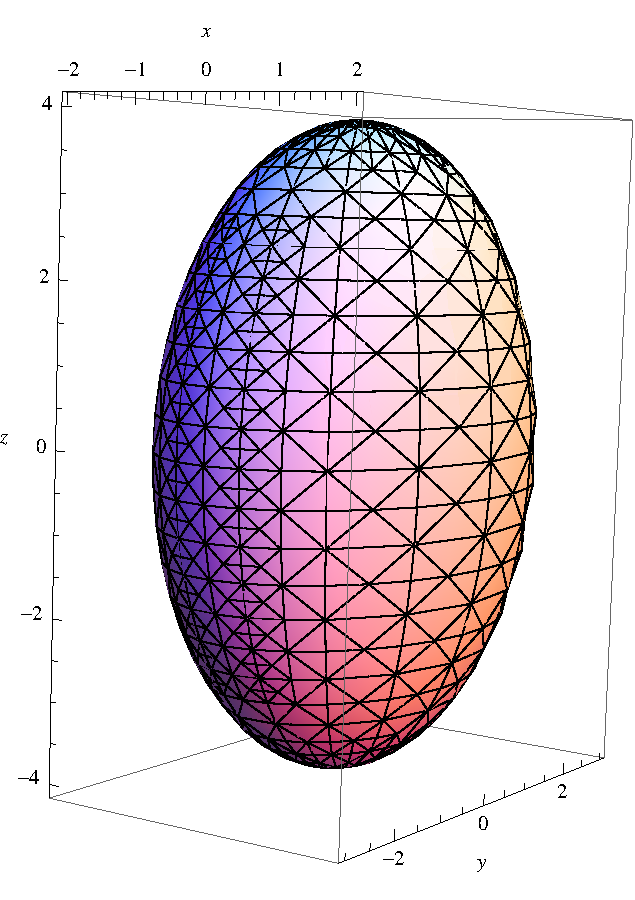
\includegraphics[scale=0.2]{images/ellipsoid.pdf}
	\columnbreak	
		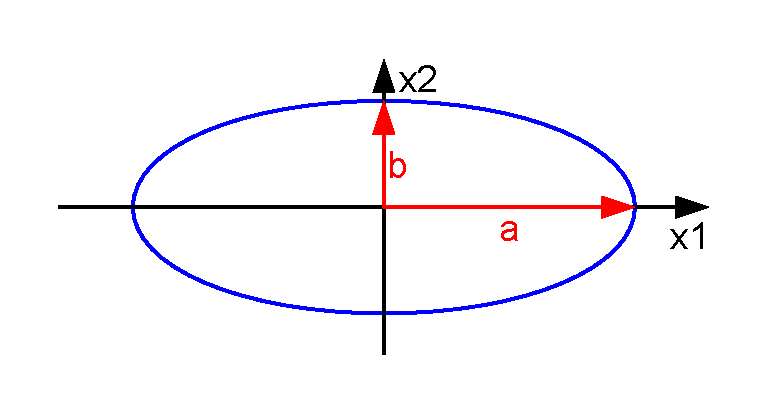
\includegraphics[scale=0.4]{images/quadrik_2d_ellipse.pdf}
\columnbreak
$$
	\sigma_{ij}=\begin{pmatrix}
		\sigma_1 & 0 & 0 \\
		0 & \sigma_2 & 0 \\
		0 & 0 & \sigma_3 \\
	\end{pmatrix}
$$
	$$\sigma_1x_1^2+\sigma_2x_2^2+\sigma_3x_3^2=1$$
	$$
	a=\frac{1}{\sqrt{\sigma_1}}; b=\frac{1}{\sqrt{\sigma_2}};
	c=\frac{1}{\sqrt{\sigma_3}}
	$$
\end{multicols}
\renewcommand{\arraystretch}{1.8}	

\begin{tabularx}{\columnwidth}{XXXX}
	\hline 
	field & law & quadric (only symmetric) & notes\\
	\hline 
	Thermal conduction &
	$j_i= -\lambda_{ij}\dfrac{\partial T}{\partial x_j} $ &
	$\lambda_1 x_1^2+\lambda_2 x_2^2+\lambda_3 x_3^2=1$ &
	$\lambda_{ij}$: therm. conductivity tensor $\lambda_{ij} = \lambda_{ji}$\newline $\rho_{ij}$: therm. resistivity tensor, $\rho_i = \dfrac{1}{\lambda_i}$\\
	
	
	\textbf{Spec Case: Heat Flow across a flow plate}&
	$\frac{\partial T}{\partial x_2}=0$ $\frac{\partial T}{\partial x_3}=0$ &	
	$
	\lambda_{11}= \lambda_1=\dfrac{j_1}{\partial T/ \partial x_1}
	$&
	temp. gradient parallel to $x_1$\\


	\textbf{Spec. case: Heat flow down a long rod(stab)} &
	$\frac{\partial T}{\partial x_1}=\rho_{11}j_1$\newline$ \frac{\partial T}{\partial x_2}=\rho_{12}j_1$\newline$ \frac{\partial T}{\partial x_3}=\rho_{13}j_1$&
	& it is recommended to work with the therm. resistance $\rho$ \\
	\hline 
	Electrical conduction & $j_i=-\sigma_{ij}\dfrac{\partial \phi}{\partial x_j}=\sigma_{ij}E_j$ \newline $j_i = \dfrac{1}{\rho_{ij}}E_i$&
	&
	$\sigma_{ij}$: electrical conductivity tensor\newline $\rho_{ij}$: electrical resistivity tensor \\
	\hline 
	Diffusion & $j_i=-D_{ij}\frac{\partial c}{\partial x_j}$&
	&
	$D_{ij}$: Diffusion tensor\\
	\hline 
\end{tabularx}
\renewcommand{\arraystretch}{1.2}	


			
	\section{Electrodynamics}
	%	\subsection{Maxwell equations}

\fcolorbox{red}{white}{

	\begin{tabularx}{\columnwidth}{llX}
		Name & Differential equations & meaning \\
		Gauss's law & $\nabla \cdot \mathbf{E} = \frac {\rho} {\varepsilon_0}$ &  The electric field in a volume is proportional to the charge inside.\\
		Gauss's law for magnetism & $\nabla \cdot \mathbf{B} = 0$ & There are no magnetic monopoles. All magnetic field lines are closed loops \\
		Induction equation & $\nabla \times \mathbf{E} = -\frac{\partial \mathbf{B}} {\partial t}$ & The voltage accumulated around a closed circuit is proportional to the time rate of change of the magnetic flux it encloses.\\
		Ampère's circuital law & $\nabla \times \mathbf{B} = \mu_0\left(\mathbf{J} + \varepsilon_0 \frac{\partial \mathbf{E}} {\partial t} \right) $& Electric currents and changes in electric fields are proportional to the magnetic field circulating about the area they pierce.\\
	\end{tabularx}
}

\subsection{Electrostatics}
	
	A direct concequence of Ampère's circuit law states the conservation of charge 
	$$  \nabla \cdot \mathbf{J} = - {\partial \rho \over \partial t} $$
	
	\renewcommand{\arraystretch}{2}
	\begin{tabularx}{\columnwidth} {lXX}
		\hline
		&point charge & distribiuted \\
		\hline
		Coulomb force&
		$\mathbf{F} = \dfrac{Q}{4\pi \varepsilon_0}\cdot \sum\limits_{i} q_i \dfrac{\mathbf{r_i}}{r_i^3}$&
		$\mathbf{F}(\textcolor{red}{\mathbf{r}}) = \dfrac{Q}{ 4\pi\varepsilon_0}\int\rho(\textcolor{darkgreen}{\mathbf{r'}}) \dfrac{\textcolor{red}{\mathbf{r}} - \textcolor{darkgreen}{\mathbf{r'}}}{|\textcolor{red}{\mathbf{r}} - \textcolor{darkgreen}{\mathbf{r'}}|^3} dV$ \\
		\hline
		Electrical Field&
		 $ \mathbf{E} = \dfrac{\mathbf{F}}{Q} = \sum\limits_i\dfrac{q_i}{4\pi\epsilon_0}\dfrac{\mathbf{r - r_i}}{|r-r_i|^3}$ &
		 $ \mathbf{E}(\textcolor{red}{\mathbf{r}}) =  \dfrac{1}{4\pi\varepsilon_0} \int \rho(\textcolor{darkgreen}{\mathbf{r'}}) \dfrac{\textcolor{red}{\mathbf{r}} - \textcolor{darkgreen}{\mathbf{r'}}}{|\textcolor{red}{\mathbf{r}} - \textcolor{darkgreen}{\mathbf{r'}}|^3}dV$ \\
		 & &  $\nabla\times\mathbf{E} = 0 \Rightarrow$ potential field $\mathbf{E}=-\nabla \varphi$\\
		\hline 
		Potential &
		$\varphi(\mathbf{r}) = \sum\limits_i \dfrac{ q_i}{4\pi\epsilon_0 |\mathbf{r}-\mathbf{r_i|}}$&
		$\varphi(r_1, r_2) = \int\limits_{r_1}^{r_2} \mathbf{E}\cdot d\mathbf{l}$\\
		\hline 
		Electric Flux & &
		$\mathbf{\Phi} = \int\limits_S \mathbf{E}\cdot\mathbf{n} dA$
		\\
		\hline 
		&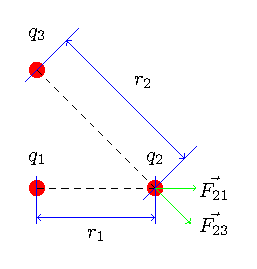
\includegraphics[scale = 1]{tikz/pointcharge.pdf} & 		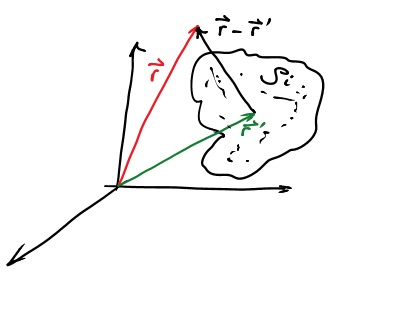
\includegraphics[width = 4cm]{images/elfield} \\
		\hline 
		Dipole formulas & $\varphi(\mathbf{r}) = \dfrac{1}{4\pi\epsilon_0}\dfrac{\mathbf{pr}}{r^3}$&
		$\mathbf{E}(\mathbf{r}) = \dfrac{1}{4\pi\epsilon_0r^3}(3\mathbf{(p\hat{r})\hat{r}-p)}$\\
		\hline 
	\end{tabularx}

	\renewcommand{\arraystretch}{1.2}

	\subsection{Electrical field in Matter}
		\begin{tabularx}{\columnwidth}{lXX}
			polarisation & $\mathbf{p} \propto \mathbf{E}$ & $p_i = \alpha_{ij}E_j$\\
			Dipole moment & $\mathbf{P} = \epsilon_0 x_{ij} E_j$ &\\
			Electrical displacement & $\mathbf{D} = \epsilon_0\mathbf{E} + \mathbf{P} = \epsilon_0 (1+\chi)\mathbf{E} = \epsilon_0\epsilon_r\mathbf{E}$&
			$D = \epsilon_0\epsilon_{ij}E_j$\\
			
		\end{tabularx}

	\subsection{Energy in the electrical field}
		{\def \arraystretch{2}	
	\begin{tabularx}{\columnwidth}{lllXX}
		&capacity & charge & work&energy density\\
		General & $C = \dfrac{Q}{U}$ & $Q = \oint\mathbf{E}d\sigma$ & $W = \int U dQ$& $w_{el} = \dfrac{W}{V}$\\
		Plate capacitor & $C = \epsilon_0\dfrac{A}{d}$ & &$W = \frac{1}{2}CU^2 = \frac{1}{2}\epsilon_0 \mathbf{E}^2A d $ & $w_{el}= \frac{1}{2}\epsilon_0\epsilon_{ij}\mathbf{E_j E_i}= \frac{1}{2}\mathbf{D_i E_i}$\\

		
	\end{tabularx}
	
		The permittivity tensor has to be symmetric: 
		$$
		\epsilon_{ij} = \begin{bmatrix}
		\epsilon_1 & 0 & 0 \\ 0 & \epsilon_2 & 0 \\ 0 & 0 & \epsilon_3 \\
		\end{bmatrix}
		$$ 

		\subsection{Magnetostatics}

		\begin{tabularx}{\columnwidth}{p{3cm}X}
		Strom       & $I = \dfrac{dQ}{dt} = \iint\limits_\epsilon \bm j d\bm A \qquad $ Stromdichte $j = \dfrac{I}{A}$\\
			
		Biot Savart & $\vec B = \dfrac{\mu_0}{4\pi}\cdot I \int \dfrac{ds\times \mathbf{r}}{r^3} = $
		$\dfrac{\mu_0}{4\pi}\iiint \bm j(\bm r') \times \dfrac{\bm r - \bm r'}{|\bm r - \bm r'|^3}dV$ \\
		flux conservation & $\nabla\cdot \mathbf{B} = 0$ all  magnetic field lines are closed\\
		Ampère law	& $\nabla\times \mathbf{B} = \mu_0 \mathbf{j}$\\
		Ohm's law			&$\bm j = \sigma \bm E\qquad \bm E =  \rho \bm j$\\
					 
		Lorentz force: point charge & $\mathbf{F} = q(\mathbf{E+v\times B})	$\\
		Lorentz force: wire  & $\bm F = I\cdot \bm l \times \bm B$\\
		
		Magnetic Moment& $\bm M = \bm m  \times \bm B \qquad  M = m  B \cdot \sin\alpha \qquad m = I A\cdot \bm n$\\
 		\end{tabularx}
	}
		\subsection{Magnetic field in Matter}
		\begin{tabularx}{\columnwidth}{lX}
			Magnetized Field & $  \mathbf{B} = \mu_0(1+ \chi_m)\mathbf{H} =  \mu_0\mu_r\mathbf{H}$	\\
		\end{tabularx}
		
		\subsection{Energy in magnetic field}
		\begin{tabularx}{\columnwidth}{lX}
			$w_{mag} = \frac{1}{2}\mathbf{BH}= \frac{1}{2}\mu_0\mu_{ij}H_j H_i$\\
		\end{tabularx}

				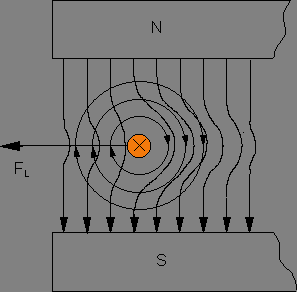
\includegraphics[scale=0.5]{images/DrahtZwischenPolen.png}
				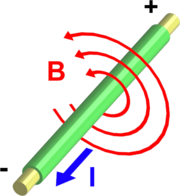
\includegraphics[scale=0.5]{images/B-Feld.png}
			$ \vec{p}=q\cdot\vec{d} $
			$ I = \sigma_{11} \cdot E_1 \cdot A $
		$ R=\rho\cdot\frac{l}{A}=\frac{1}{\sigma} \cdot\frac{l}{A}$\\

		\begin{tabular}{|c|c|}
				\hline Strom & Daumen \\ 
				\hline B-Feld & Zeigefinger \\ 
				\hline Kraft & Mittelfinger \\ 				
				\hline
			\end{tabular} 
			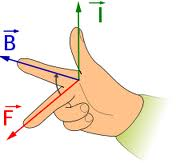
\includegraphics[scale=0.5]{images/handregel.jpg}	
			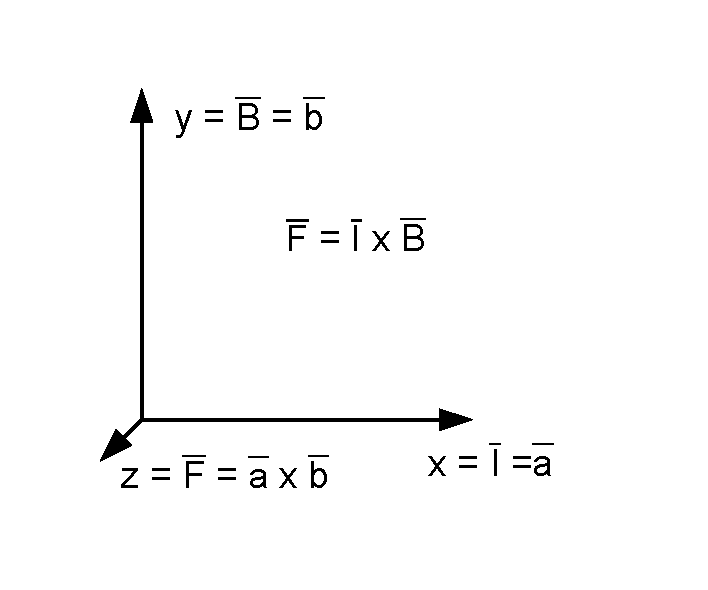
\includegraphics[scale=0.5]{images/kreuzprodukt.pdf}


	\section{Elasticity}
    		\subsection{Elasticity in 1D}
\renewcommand{\arraystretch}{2.2}
	\begin{tabularx}{ \columnwidth} {p{3cm}XlX}
		\hline 
		\multicolumn{4}{p{\columnwidth}}{Stored momentum sets an object into motion. If the object doesn't move, but a momentum is applied, the object deforms.}\\
		Hook's Law & $F = k\cdot \Delta u$ &
		momentum   & $p = m\cdot v$\\
		
		momentum flux & $J_p = \dfrac{\partial p}{\partial t}$&
		momentum flux density & $j_p = \dfrac{J_p}{A}$\\
		
		mechanical stress (Spannung) & $\sigma_{11} = -j_p = \frac{-J_p}{A} $ &
		cutting force, flux of momentum & $F = \int_A \sigma_{11} dA$\\
		mechanical strain (Elastizität) &$\varepsilon_{11} = \dfrac{\partial u(x)}{\partial x}$&
		Youngs Modulus (Eleastizitätsmodul) &  $E = \dfrac{\sigma_{11}}{\varepsilon_{11}} $\\		
		Young Modulus & $F = \dfrac{EA_0\Delta L}{L_0}$&&\\
		\hline 
		\textbf{Momentum Balance equation} & $\dfrac{\partial \sigma_{11}}{\partial x} + \rho g= 0$ &
		boundary cond. & $\sigma_{11}(0) = \dfrac{F}{A} \newline  \sigma_{11}(L) = 0$ \\
		
		Displacement Field & $u(x) = \Delta u \cdot \dfrac{x}{L}$ & 
		$u(L) = \Delta x$ &  u(0) = 0 \\
		Material Law & $\varepsilon_{11}$\newline $ E $\\ 
		
	\end{tabularx}
\renewcommand{\arraystretch}{1.2}	
	 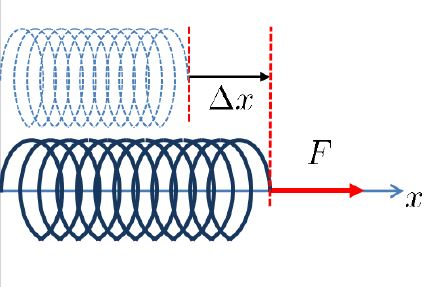
\includegraphics[scale = 0.3]{images/hook}
		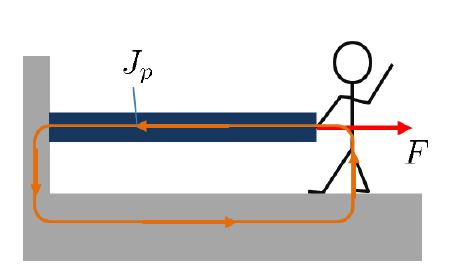
\includegraphics[scale=.3]{images/momentcons}
		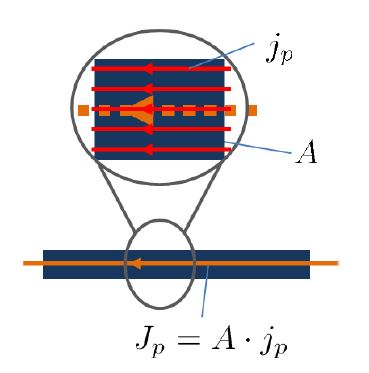
\includegraphics[scale=.3]{images/momflux}
		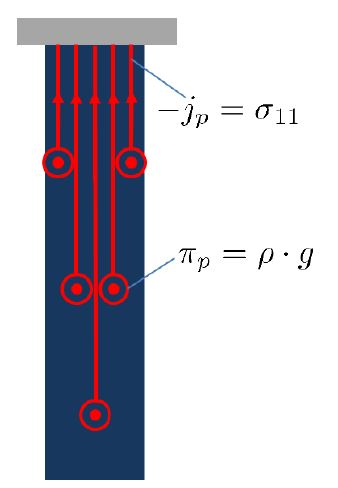
\includegraphics[scale=.3]{images/momfluxdensity}
		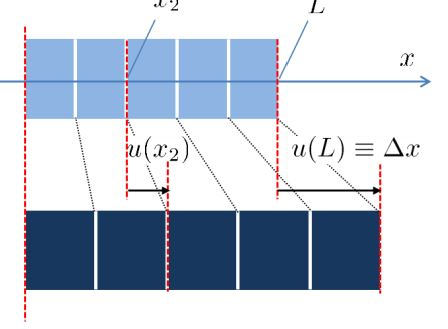
\includegraphics[scale=.3]{images/strain}
%		\includegraphics[scale=.3]{images/}				


\begin{tabularx}{\columnwidth}{p{3cm}XX}
	\hline 
	\multicolumn{3}{c}{Elasticity in a hanging rope}\\
	\hline 
	\multicolumn{3}{l}{The Rope is hanging from the ceiling in the gravitational Field of the earth}\\
	
	measured values& $L, A,\rho, E, g$ & \\
	mechanical stress & $\dfrac{\partial \sigma}{\partial x}  + \rho g = 0 \qquad \sigma(x) = -\rho g x + C$ & $\sigma(0) = \dfrac{F}{A} = \dfrac{mg}{A} = \dfrac{mgL}{AL} = L\rho g$\\
	&$\sigma(0) =\rho g L \qquad \sigma(x)  = \rho g(L-x)$ &
	$\sigma(x) = \varepsilon(x) E = \dfrac{\partial u(x)}{\partial x}E = \rho g(L-x)$\\
	strain & $\varepsilon(x)= \dfrac{\rho g}{E}(L-x)$ & $u(x) = \int \varepsilon(x)dx = \dfrac{\rho g}{E}(Lx-\dfrac{x^2}{2}+C)$\\
	Displacement Field& $u(0) = 0 \quad u(x) =\dfrac{\rho g}{E}(Lx-\dfrac{x^2}{2})$ & \\
	maximal stress & $\sigma_{max} = \rho g L$ \hspace{1.3cm}maximal elongation&  $\dfrac{\partial u}{\partial x} = 0 \Rightarrow  x_{max} = L \quad u_{max} = \dfrac{\rho g}{2E}L^2$\\

	\hline 
	\multicolumn{3}{c}{calculating a spring constant}\\
	\hline 
	measured values & $L, A, E$&\\
	& $\sigma = \dfrac{F}{A} = \text{const} \quad u(x) = \dfrac{F}{AE}x$ & elongation for $x=L \quad \Delta u = \dfrac{FL}{AE}$\\
	spring const. & $F = k\cdot \Delta u$ & $k = \dfrac{AE}{L}$\\
	\hline 
	
\end{tabularx}
\newpage

\subsection{Elasticity in 3D}
	electrodyamics: scalar charge $q$ $\Rightarrow$ vectorial flux $j$ (0 rank tensor $\Rightarrow$ 1st rank tensor)
	
	mechanics: vector momentum $\mathbf{p}$ $\Rightarrow$ tensorial flux density $\mathbf{\sigma}$ (1st rank tensor $\Rightarrow$ 2nd rank tensor)

%	$$
%	\sigma = \begin{pmatrix}
%	\sigma_{11} & \sigma_{12} & \sigma_{13} \\
%	\sigma_{21} & \sigma_{22} & \sigma_{23} \\
%	\sigma_{31} & \sigma_{32} & \sigma_{33} 
%	\end{pmatrix}
%	$$

\begin{tabularx}{ \columnwidth} {p{4cm}lX}
	\hline 
	General momentum balance equation &  $\dfrac{\partial \sigma_{ik}}{\partial x_k} + \rho g_i = 0$ & $\sigma_{ij}$: stress tensor of 2nd rank, characterizes material symmetry: $\sigma_{ij} = \sigma_{ji}$\\
	Cutting Force & $F_i^\alpha = \sigma_{ik} nA^\alpha_k \cdot A^\alpha$ & $\mathbf{n}^\alpha$: normal vector pointing outside of the cuboide\newline $A^\alpha$: face area 
	\\
	
	Angular Momentum &
	$\mathbf{M} = 0 $ &
	\\
	Stress Decomposition &  $\sigma^{iso}=\frac{\operatorname{tr} \sigma}{3} \cdot \mathbb{I} \equiv \frac{1}{3} \mathbb{E} : \varepsilon$ 
	&$\sigma^{shear}= \left(\mathbb{I}- \frac{1}{3}\mathbb{E} \right) : \varepsilon\qquad $ 
	$\sigma^{shear} = \sigma -\sigma^{iso}$\\ 
	
	$\begin{pmatrix}
	x\to x & x\to y & x\to z \\
	y\to x & y\to y & y\to z \\
	z\to x & z\to y & z\to z \\		
	\end{pmatrix}$&
	\multicolumn{2}{l}{\vspace{0cm}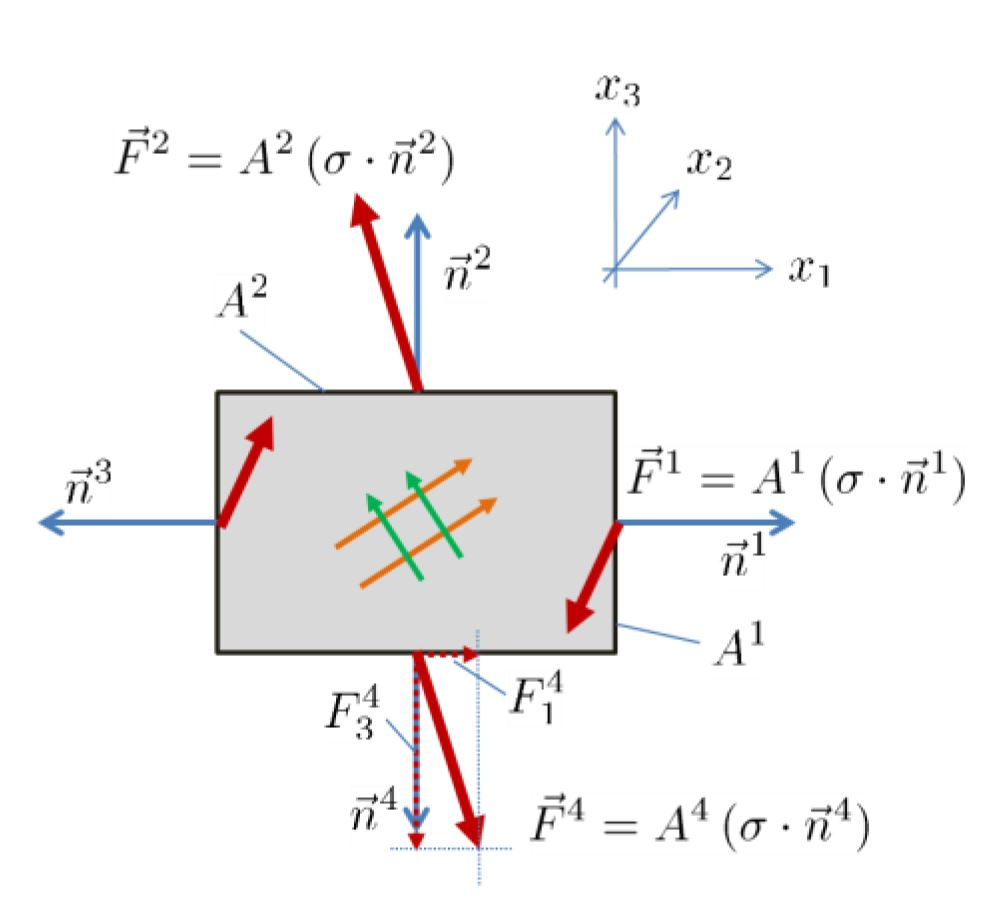
\includegraphics[scale=.15]{images/3Dcuttingforces} 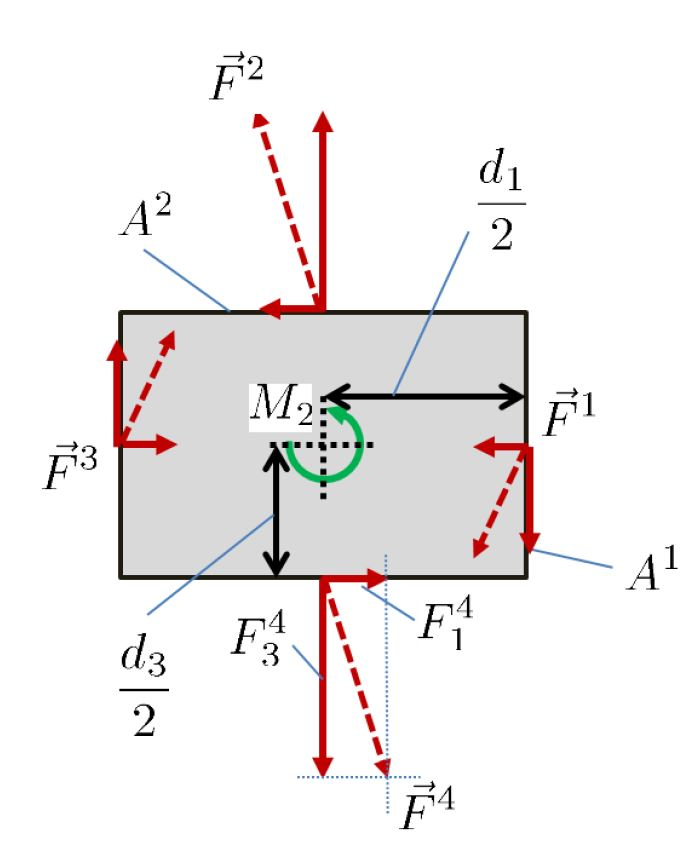
\includegraphics[scale=.15]{images/3Dangularmomentum}}	\\
	\hline 
\end{tabularx}
	\renewcommand{\arraystretch}{2}
\subsection{Special Stress States (Mechanische Spannung $\sigma = F/A$)}
	\begin{tabularx}{\columnwidth}{p{2cm}p{2cm}XX}
		\hline 
		Stress State & Tensor law & matrix notation & \\ 
		\hline 
		Isotropic Stress State & $\sigma_{ij} = -P\delta_{ik}$&	$ \sigma = \begin{pmatrix} -P & 0 & 0\\ 0 & -P & 0\\ 0 & 0 & -P \end{pmatrix}$ &\vspace*{-1.2cm}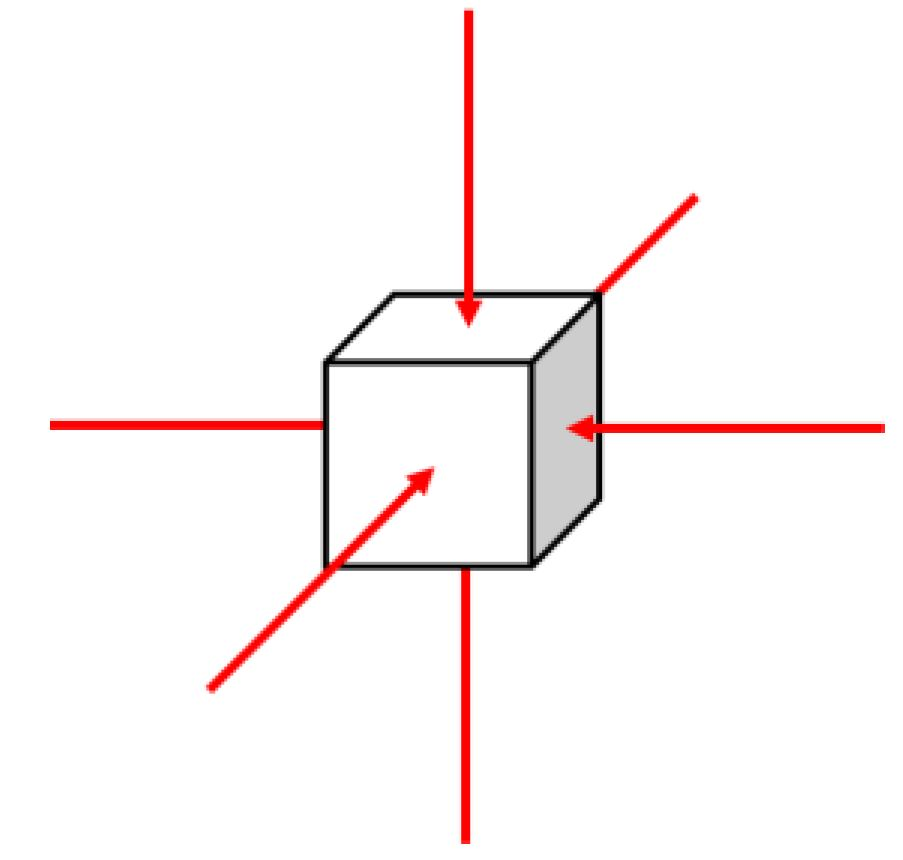
\includegraphics[scale=.11]{images/3Dcfisotropic}\\
		\hline 
		Uniaxial Stress State & & 		$ \sigma = \begin{pmatrix} \sigma_{11} & 0 & 0\\ 0 & 0 & 0\\ 0 & 0 & 0\\ \end{pmatrix}$ &		\vspace*{-1.2cm}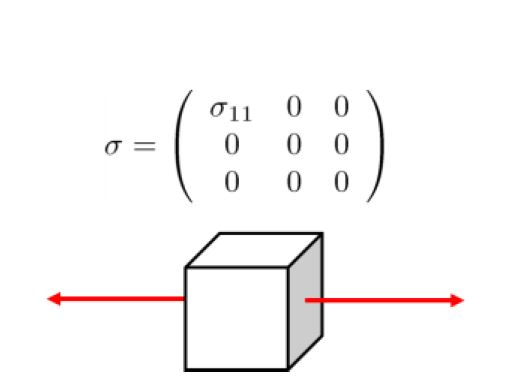
\includegraphics[scale=.12]{images/3Dcfuniaxial}\\
		\hline 
		Plane Stress State && $ \sigma = \begin{pmatrix} \sigma_{11} & \sigma_{12} & 0\\ \sigma_{21} & \sigma_{22} & 0\\ 0 & 0 & 0\\ \end{pmatrix}$&	\vspace*{-1.0cm}	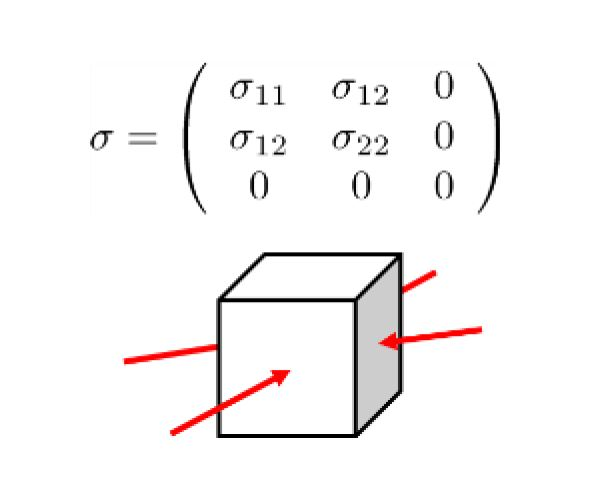
\includegraphics[scale=.12]{images/3Dcfplanestress}\\
		\hline 
		Principal Axis Decompensation &&$ \sigma = \begin{pmatrix} \sigma_{11} &  0& 0\\ 0 & \sigma_{22} & 0\\ 0 & 0 & \sigma_{33}\\ \end{pmatrix}$&\\
		\hline 
		Pure Shear Stress State &$\operatorname{tr}\sigma = 0$&$ \sigma = \begin{pmatrix} 0 &  -s& 0\\ -s & 0 & 0\\ 0 & 0 & 0\\ \end{pmatrix}$&		\vspace*{-1.2cm}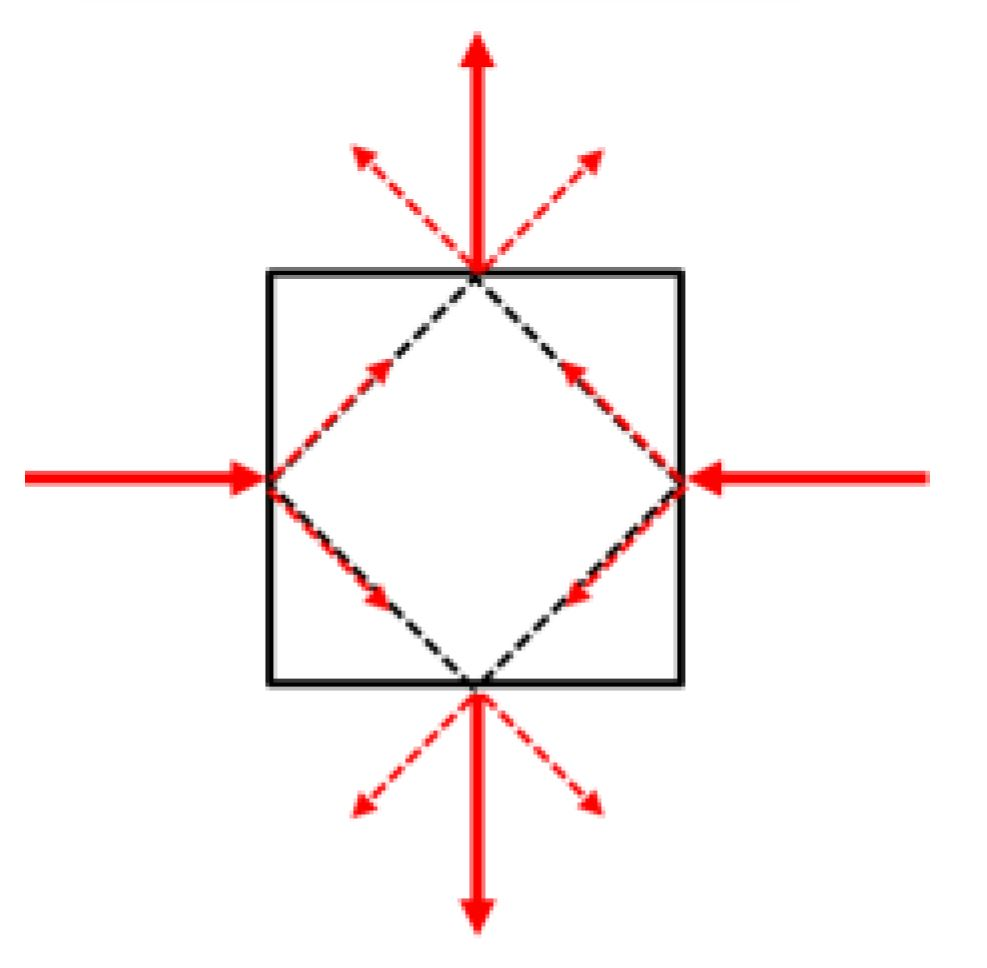
\includegraphics[scale=.12]{images/3Dcfpureshear}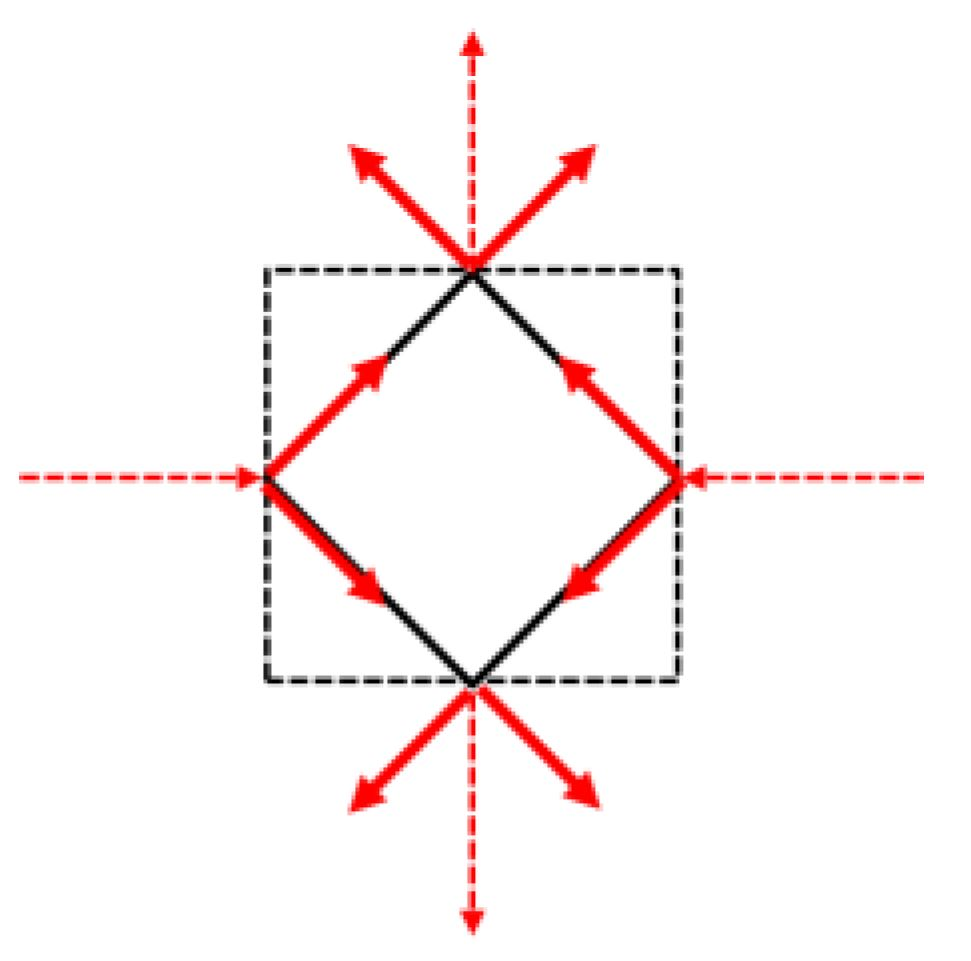
\includegraphics[scale=.12]{images/3Dcfpureshear2}\\
		\hline 
	\end{tabularx}
	\renewcommand{\arraystretch}{1.2}

\subsection{Strain Tensor in 3D}
	Vector of 2nd rank. Gradient of Deformation $u(x)$ \hspace{1cm}$\bm x' = \bm x + \bm u(\bm x)$
	
	\begin{tabularx}{\columnwidth}{p{2cm}XX}
		\hline 
		   $e_{ij} = \dfrac{\partial u_i}{\partial x_j}$&
			$e = \begin{pmatrix}
			\frac{\partial u_1}{\partial x_1} & \frac{\partial u_1}{\partial x_2} &
			\frac{\partial u_1}{\partial x_3}\\
			\frac{\partial u_2}{\partial x_1} & \frac{\partial u_2}{\partial x_2} &
			\frac{\partial u_2}{\partial x_3}\\
			\frac{\partial u_3}{\partial x_1} & \frac{\partial u_3}{\partial x_2} &
			\frac{\partial u_3}{\partial x_3}\\
			\end{pmatrix}$ &
			\vspace*{-.5cm}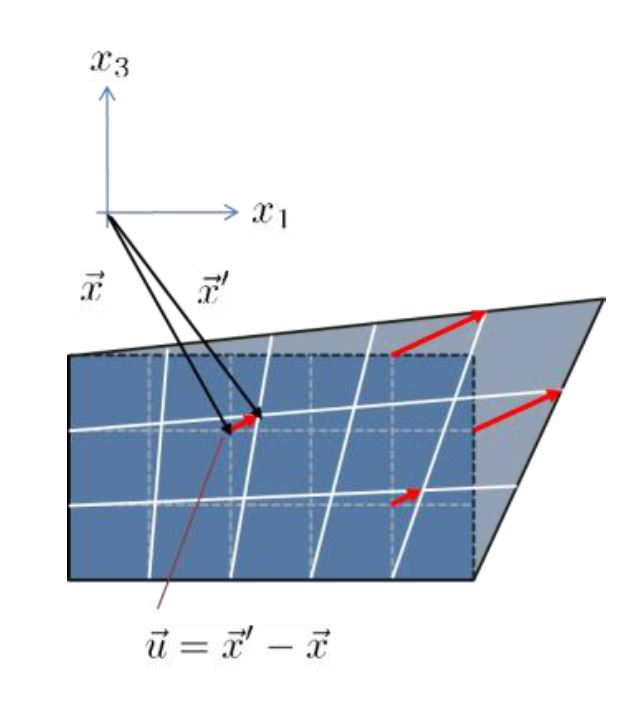
\includegraphics[scale=.2]{images/2Ddeformation}\\
			
			&
			\multicolumn{2}{l}{$\bme = \bme^{sym} + \bme^{anti} = \frac{1}{2}(\bme+\bme^T) + \frac{1}{2}(\bme - \bme^t)$ }\\

			strain tensor & $\varepsilon = \bme^{sym} = \frac{1}{2}(\bme+\bme^T)= \frac{1}{2} (\frac{\partial u_i}{\partial x_j} + \frac{\partial
				u_j}{\partial x_i})$  &\\
			\multicolumn{2}{l}{rotational deformation} & $\gamma = \bme^{anti} = \frac{1}{2}(\bme-\bme^T)$ \\
			\hline
			\multicolumn{3}{c}{\textbf{Rigid body transformation (rigid = starr)}}\\
			\multicolumn{3}{c}{Rigid body transformations do not mechanically deform the body. }\\
			rigid transformation &   
			$x' = x + u(x) \quad u_i(x) = (R_{ij} - \delta_{ij})x_j$ & $R_{ij}$: rotation matrix\\
			&  $\bme \approx \begin{pmatrix} 0 & -\phi &0 \\ \phi &  0& 0 \\  0& 0 & 0\\	\end{pmatrix}$ &
			antimsymmetric deformation tensors correspond to small rotations and don't produce stress within the body\\

			\hline 
			\multicolumn{3}{c}{\textbf{Examples of Strain States}}\\			
			Volume Change of a Deformation & $\dfrac{\Delta V}{V} = \operatorname{tr} \varepsilon$ &
			\vspace*{-.5cm} 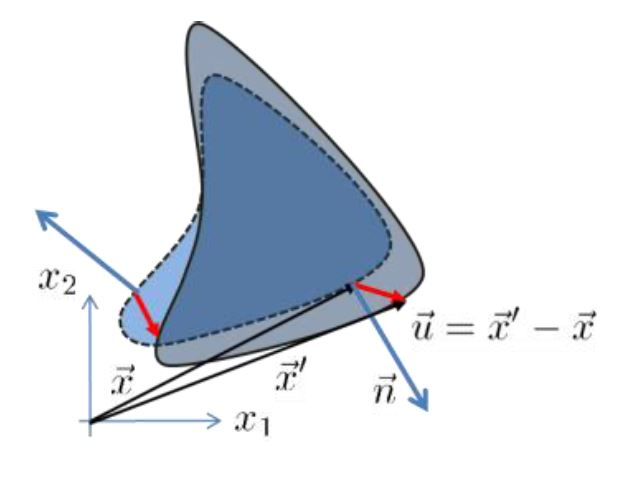
\includegraphics[scale=.2]{images/deformvolume}\\
			\hline 
			pure shear strain & $\operatorname{tr}\varepsilon = 0$ & no volume change\newline only shape chanign\\
			\hline 
			Isotropic Strain &$\varepsilon_{11}=\varepsilon_{22}=\varepsilon_{33}\quad$
			$\varepsilon_{ij} = \varepsilon \cdot \delta_{ij} \qquad \dfrac{\Delta V}{V} = 3\varepsilon_{11}$ & volume changing\newline form of the body stays the same\\
			\hline 
			Plain strain &  $\varepsilon_{33} = \varepsilon_{13} = \varepsilon_{23}= 0$ => $\varepsilon =
				\begin{pmatrix}
				* & * & 0\\
				* & * & 0\\
				* & * & 0\\
				\end{pmatrix} $ &
				No deformation in z axis\\
			\hline 
			Strain Decomposition &   $\varepsilon^{iso}=\frac{\operatorname{tr} \varepsilon}{3} \cdot \mathbb{I} \equiv \frac{1}{3} \mathbb{E} : \varepsilon$&
			$\varepsilon^{shear} = (\mathbb{I} - \frac{1}{3}\mathbb{E}): \varepsilon$\\
			&
			$\varepsilon = \varepsilon^{iso} + \varepsilon^{shear}$ &
			\\
			\hline 

	\end{tabularx}
\newpage
\subsection{Isotropic Mechanical Material Laws}
	\begin{tabularx}{\columnwidth}{p{3cm}XX}
		\hline 
		 \multicolumn{2}{p{10cm}}{$\mathbb{C}^{iso} = K \cdot \mathbb{E} + 2G \cdot (\mathbb{I} - \frac{1}{3}
		 \mathbb{E}) =  (K - \frac{2}{3} G) \cdot \mathbb{E} + 2G \cdot \mathbb{I}$ } &
		 K: bulk modulus(Kompressionsmodul) \newline G: shear modulus(Schubmodul)\\
		 &mostly: $K \gg G$ &\\
		 \hline 
		 \multicolumn{3}{c}{Elasticity Tensor 
		 	$\mathbb{C}^{eng} = K \cdot \begin{pmatrix}
		 		1 & 1 & 1 & 0 & 0 & 0\\
		 		1 & 1 & 1 & 0 & 0 & 0\\
		 		1 & 1 & 1 & 0 & 0 & 0\\
		 		0 & 0 & 0 & 0 & 0 & 0\\
		 		0 & 0 & 0 & 0 & 0 & 0\\
		 		0 & 0 & 0 & 0 & 0 & 0\\
		 	\end{pmatrix}
		 	+ 2 G \cdot \begin{pmatrix}
		 		\frac{2}{3} & -\frac{1}{3} & -\frac{1}{3} & 0 & 0 & 0\\
		 		-\frac{1}{3} & \frac{2}{3} & -\frac{1}{3} & 0 & 0 & 0\\
		 		-\frac{1}{3} & -\frac{1}{3} & \frac{2}{3} & 0 & 0 & 0\\
		 		0 & 0 & 0 & \frac{1}{2} & 0 & 0\\
		 		0 & 0 & 0 & 0 & \frac{1}{2} & 0\\
		 		0 & 0 & 0 & 0 & 0 & \frac{1}{2}\\
		 	\end{pmatrix}$}\\
		 \hline 
		 
		Material reaction to pure compression & $\sigma_{ij}^{comp} = C_{ijkl}^{iso}\varepsilon_{kl}^{comp} = -K\kappa\cdot\delta_{ij}$ & K express material reaction to pure compression\\
		\hline 
		Material reaction to pure Shear Deformation & 
		$\varepsilon_{ij}^{shear} = C_{ijkl}^{iso}\varepsilon_{kl}^{shear} = 2G\varepsilon_{ij}^{shear} $&
		G express material reaction to pure shear compression\\
		\hline 
		Uniaxial stress &
		\multicolumn{2}{p{12cm}}{
		$\begin{pmatrix}
			\sigma_{11}\\
			0\\
			0
		\end{pmatrix} = 
		\begin{pmatrix}
			K + \frac{4G}{3} & K - \frac{2G}{3} & K - \frac{2G}{3}\\
			K - \frac{2G}{3} & K + \frac{4G}{3} & K - \frac{2G}{3}\\
			K - \frac{2G}{3} & K - \frac{2G}{3} & K + \frac{4G}{3}\\
		\end{pmatrix}\cdot
		\begin{pmatrix}
			\varepsilon_{11}\\
			- \varepsilon_{22}\\
			- \varepsilon_{33}
		\end{pmatrix}\qquad
		\sigma_{11} = E\cdot \varepsilon_{11}$ } \\
	\hline 
	Poisson's ration & $\nu = -\dfrac{\varepsilon_{22}}{\varepsilon_{11}} = -\dfrac{\varepsilon_{33}}{\varepsilon_{11}}=\dfrac12 \cdot \dfrac{3K -2G}{3K+G}$&
	ratio of dilation and elongation under uniaxial stress\\
	Young's modulus & $E = \dfrac{\sigma_{11}}{\varepsilon_{11}} = \dfrac{9KG}{3K + G}$&\\
	\hline 
	& \multicolumn{2}{l}{
				$\mathbb{C}^{eng} = \frac{E}{1 + \nu} \cdot \begin{pmatrix}
					\frac{1-\nu}{1-2\nu} & \frac{\nu}{1-2\nu} & \frac{\nu}{1-2\nu} & 0 & 0 & 0\\
					\frac{\nu}{1-2\nu} & \frac{1-\nu}{1-2\nu} & \frac{\nu}{1-2\nu} & 0 & 0 & 0\\
					\frac{\nu}{1-2\nu} & \frac{\nu}{1-2\nu} & \frac{1-\nu}{1-2\nu} & 0 & 0 & 0\\
					0 & 0 & 0 & \frac{1}{2} & 0 & 0\\
					0 & 0 & 0 & 0 & \frac{1}{2} & 0\\
					0 & 0 & 0 & 0 & 0 & \frac{1}{2}\\
				\end{pmatrix}$}\\
		\hline 
	Plane Strain  	 & $\epsilon_{i3} = 0 $\newline damn is an example of such a state& 
	strain Tensor $\varepsilon^{eng} = (\varepsilon_{11}, \varepsilon_{22}, 2\varepsilon_{12})^T$\\
	&$\mathbb{C}^{eng} = \dfrac{E}{1+\nu}\cdot  \begin{pmatrix}
	\dfrac{1-\nu}{1-2\nu} & \dfrac{\nu}{1-2\nu} & 0\\
	\dfrac{\nu}{1-2\nu} & \dfrac{1-\nu}{1-2\nu} & 0\\
	0 & 0 & \dfrac{1}{2}\\
	\end{pmatrix}$&
	$\sigma^{eng} = \mathbb C^{iso,eng}\varepsilon = (\sigma_{11},\sigma_{22}, \sigma_{12})^T$
	\\
	\hline 
	
	Plane Stresss & 
	$\sigma_{i3} = 0$ & 
	\\
	&
	$\mathbb{C}^{eng} = \dfrac{E}{1+\nu}\cdot\begin{pmatrix}
		\dfrac{1}{1-\nu} & \dfrac{\nu}{1-\nu} & 0\\
		\dfrac{\nu}{1-\nu} & \dfrac{1}{1-\nu} & 0\\
		0 & 0 & \dfrac{1}{2}\\
	\end{pmatrix}$
	&\\
	\hline 
	\end{tabularx}


%		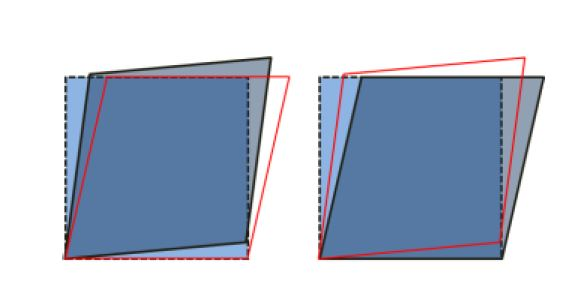
\includegraphics[scale=.3]{images/deformgrad}

%		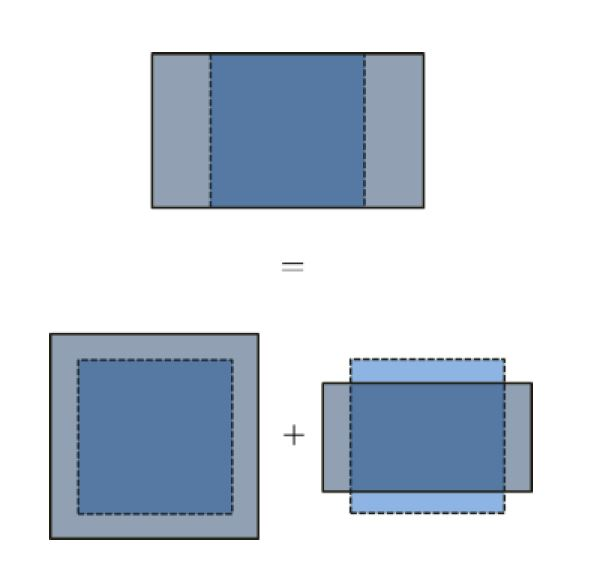
\includegraphics[scale=.3]{images/allstates}
%		\includegraphics[scale=.3]{images/}





	\section{Examples}
	%		\section{balance equation}
	\subsubsection{Ohm's Law}
		% Exercise Chapter 1, Aufgabe 2
		...bitte noch übertragen...
		\subsubsection{Heat conduction in 1D}
		% Exercise Chapter 1, Aufgabe 3
		\begin{itemize}
			
			\item Formulate the stationary het balance equation for a 1D system (slender rod). Genommen wird die Allgemeine Wärmeleitungsgleichung $\frac{\partial w}{\partial t}= -\nabla \cdot j_W+q_W$ und diese Vereinfacht, da Stationär und 1D ergibt es $0= -\frac{\partial j_W}{\partial x}+q_W$
			
			\item Formulate Fourier's law of heat conduction in 1D. Dies ist Allgemein $j_W=-\lambda \cdot \nabla T$ und im 1D $j_W=-\lambda \frac{\partial T}{\partial x} T$
			
			\item Solve this system of 2 ODEs of $1^{st}$ order for following conditions: a Al rod of length L=20cm , cross section $A=1cm^2$ and specific heat conductivity 
			$ \lambda = 240 W/(Km) $ 
			is cooled to $25^\circ C$ on its right hand side and heated on the lhs with a heat flux density of $ 36 kW/m^2 $ (candle).
			Es gilt das Fourier's law in die balance equation einzusetzen ergibt $ 0=\lambda \frac{\partial^2T}{\partial x^2}+q_W$, da es keine Quelle oder Senke hat gilt $q_W=0$. Löst man diese Differentialgleichung ergibt es $T(x)=C_1x+C_2$. An der Stelle (x=0) gilt das Fourier's law, also gilt $j_W=-\lambda \frac{\partial T}{\partial x} = 36000 = -240 \frac{\partial T}{\partial x } \Rightarrow \frac{\partial T}{\partial x}=-150 \frac{K}{m} =C_1$ und auch gegeben ist $25^\circ C$ an der Stelle x=0.2m. Damit $C_2$ ausrechnen ergibt  $ T(0.2)= -150 \frac{K}{m} \cdot 0.2m+C_2=25^{\circ} C $. Allgemein ergibt sich die Gleichung $ T(x)= -150 \frac{K}{m} \cdot x [m] + 25^{\circ} C $.
			
			\item Neu sind beide Seiten sind $25^\circ K$ Nun kommt zusätzlich noch eine Wärmequellerate für $500 kW/m^3$ nun gibt es $ -\lambda \frac{\partial^2T}{\partial x^2}=q_W$ löst man diese Partielle DGL ergibt es $T(x)=\frac{1}{2}\frac{-q_W}{\lambda} x^2+C_1x+C_2$ Setzt man die Randbedingungen ein ergibt es $T(x)=\frac{1}{2}\frac{q_W}{\lambda}(Lx-x^2)+T_0$
			
			
		\end{itemize}



	\subsubsection{Gauss Theorem}
	kubischer Würfel [1m, 1m, 1m] in 3d\\
	Vektorfeld: $v = v_0 (\frac{x_1}{a}, \frac{x_2}{a}, 0)^T$ mit $v_0 = 0.1 m/s$
	und $a = 1m$\\
	
	\textbf{sketch flow field in $x_1$, $x_2$-plane}\\
	
	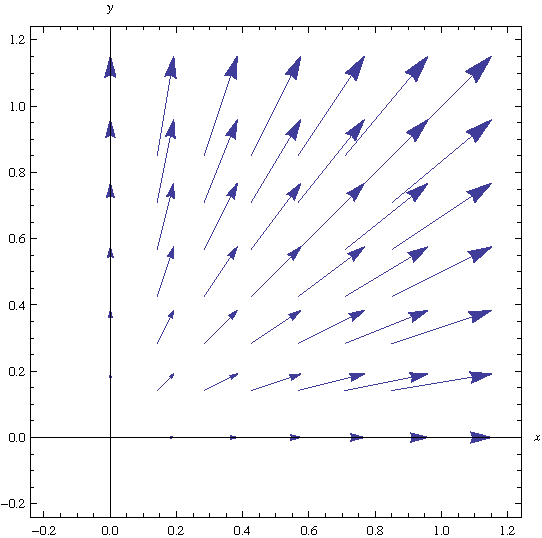
\includegraphics[scale=0.5]{images/gauss.pdf}\\ % weg mit dem figure plunder
	Vectorfield\\
	
	
	\textbf{Fluss über Fläche berechnen}\\
	Fluss über alle Flächen summieren:\\
	Fläche unten $x_1$,$x_3$ bei $x_2 = 0$:
	\begin{align}
		\oint_{S} \vec u \cdot
		\vec n\; \mathrm dA = \frac{v_0}{a} \oint_{S} \begin{pmatrix}
			x_1\\ x_2\\ 0
		\end{pmatrix} \cdot
		\begin{pmatrix}
			0\\ -1\\ 0
		\end{pmatrix} \mathrm dA = \frac{v_0}{a} \int_{0}^{1} \int_{0}^{1} x_2 \mathrm
		dx_1 \mathrm dx_3 = \frac{v_0}{a} \int_{0}^{1} \int_{0}^{1} 0 \mathrm dx_1
		\mathrm dx_3 = 0
	\end{align}
	Fläche oben $x_1$,$x_3$ bei $x_2 = 1$:
	\begin{align}
		\oint_{S}
		\vec n\; \mathrm dA = \frac{v_0}{a} \oint_{S} \begin{pmatrix}
			x_1\\ x_2\\ 0
		\end{pmatrix} \cdot
		\begin{pmatrix}
			0\\ -1\\ 0
		\end{pmatrix} \mathrm dA = \frac{v_0}{a} \int_{0}^{1} \int_{0}^{1} x_2 \mathrm
		dx_1 \mathrm dx_3 = \frac{v_0}{a} \int_{0}^{1} \int_{0}^{1} 1 \mathrm dx_1
		\mathrm dx_3 = \frac{v_0}{a}
	\end{align}
	Fläche hinten $x_1$,$x_2$ bei $x_3 = 1$:
	\begin{align}
		\oint_{S} \vec u \cdot
		\vec n\; \mathrm dA = \oint_{S} \frac{v_0}{a} \begin{pmatrix}
			x_1\\ x_2\\ 0
		\end{pmatrix} \cdot
		\begin{pmatrix}
			0\\ 0\\ 1
		\end{pmatrix} \mathrm dA = \int_{0}^{1} \int_{0}^{1} 0 \mathrm dx_1 \mathrm
		dx_2 = 0
	\end{align}
	Sinngemäss für alle Flächen Durchziehen:
	\begin{align}
		I_{tot} = \frac{v_0}{a} + \frac{v_0}{a} + 0 + 0 + 0 + 0 = 2 \frac{v_0}{a}
	\end{align}
	
	Mit Gauss theorem über Fläche (einfacher):
	\begin{align}
		\int_V \nabla \vec u \; \mathrm dV = \int_V \nabla \begin{pmatrix}
			x_1\\ x_2\\ 0
		\end{pmatrix} \; \mathrm dV = \int_{V}
		\frac{\partial x_1}{\partial x_1} + \frac{\partial x_2}{\partial x_2} +
		\frac{\partial 0}{\partial x_3} \; \mathrm dV =
		\frac{v_0}{a}
		\int_{0}^{1}
		\int_{0}^{1}
		\int_{0}^{1} 1 + 1 + 0 \; \mathrm dx_1 \mathrm dx_2 \mathrm dx_3 = 2
		\frac{v_0}{a}
	\end{align}

\subsubsection{Elastic Energy Density} % Probeprüfung Aufgabe 5

Der Tensor $ \epsilon^{eng}=(1,-1,1,2,0,0)^T $ aufteilen in $ \epsilon^{iso} $ und $ \epsilon^{shear} $. 
\\
Man übersetzt den Tensor von eng Notation in einen normalen Tensor. 
\\
$ \epsilon^{ing}
=
\begin{pmatrix} 
1 \\ 
-1 \\
1 \\ 
2 \\
0 \\ 
0 \\ 
\end{pmatrix}
\rightarrow 
\begin{pmatrix} 
1 & 0 & 0 \\
0 & -1 & 1 \\
0 & 0 & 1 \\
\end{pmatrix}
=
\epsilon $
\\
Nun gilt es den Tensor $ \epsilon $ aufzuteilen
\\
$ \epsilon^{iso}=\frac{tr(\epsilon)}{3}\cdot \textbf{I} = \frac{1}{3}\cdot
\underbrace{tr\begin{pmatrix} 
	1 & 0 & 0 \\
	0 & -1 & 1 \\
	0 & 0 & 1 \\
	\end{pmatrix}}_1
\cdot
\begin{pmatrix} 
1 & 0 & 0 \\
0 & 1 & 0 \\
0 & 0 & 1 \\
\end{pmatrix}
\rightarrow
\epsilon^{eng}_{iso}=
\frac{1}{3}\cdot
\begin{pmatrix} 
1 \\ 
1 \\
1 \\ 
0 \\
0 \\ 
0 \\ 
\end{pmatrix}
$
\\
$ \epsilon^{shear}=\epsilon-\epsilon^{iso}=
\begin{pmatrix} 
1 & 0 & 0 \\
0 & -1 & 1 \\
0 & 0 & 1 \\
\end{pmatrix}
-
\frac{1}{3}
\begin{pmatrix} 
1 & 0 & 0 \\
0 & 1 & 0 \\
0 & 0 & 1 \\
\end{pmatrix}
=
\frac{1}{3}
\begin{pmatrix} 
2 & 0 & 0 \\
0 & -4 & 1 \\
0 & 0 & 2 \\
\end{pmatrix}
=
\frac{1}{3}\cdot
\begin{pmatrix} 
2 \\ 
-4 \\
2 \\ 
6 \\
0 \\ 
0 \\ 
\end{pmatrix}
\rightarrow
\epsilon^{ing}_{shear}
\frac{1}{3}\cdot
\begin{pmatrix} 
2 \\ 
-4 \\
2 \\ 
6 \\
0 \\ 
0 \\ 
\end{pmatrix}
$

\subsubsection{2nd Rank Tensor Manipulation} % Exercises of Chapter 3

a) $\mathbf{C}=\mathbf{AB}$ $\Rightarrow$ $C_{ij}=A_{ik}B_{kj}$

Matrixmulitplikation weil die Dimension des resultierenden Tensors aus der
Anzahl Spalten des linken Tensors und der Anzahl Zeilen des Rechten Tensors
besteht. \qed

b) General heat conduction law $j_{th,k}=-\kappa_{kl}\frac{\partial
	T}{\partial x_l}$ Prove that the isotropic law is recovered by using the
specific 2nd Rank Tensor $\kappa_{kl}=\kappa \delta_{kl}$

$K_{kl}$ Einsetzen. In diesem Fall ist das Korneckerdelta eine $1$. Deshalb
ergibt sich $-\kappa \frac{\partial T}{\partial x_k}$ \qed

c) Show that the 2nd Rank Unit Tensor $\mathbf{I}$ has the same form in each
coordinate system.$\Rightarrow$ Orthogonal

Transformation eines Einheitstensors: $\mathbf{I}'=R\mathbf{I}R'\Rightarrow$.
$I_{il}'=R_{ij}\delta_{jk}R_{kl}^T = R_{ij}R_{jl}^T=\delta_{il}=I_{il}$ \qed



d) Prove tr $\mathbf{E}=\mathbf{E : I}$
Component $\Rightarrow$ $E_{ij}\delta_{ij}=E_{ii}$ \qed

e) Prove every 2nd Rank can be written as symmetric and asymmetric tensor.

$\mathbf{A}=\frac{1}{2}\left(\mathbf{A} + \mathbf{A}^T\right)+
\frac{1}{2}\left(\mathbf{A}-\mathbf{A}^T\right) = \mathbf{A}$ \\
$\mathbf{A}=\left(\mathbf{A}_1^{sym}-\mathbf{A}_1^{sym}\right)=\left(\mathbf{A}_2^{sym}-\mathbf{A}_2^{sym}\right)$
\\
$0=\left(\mathbf{A}_1^{sym}-\mathbf{A}_2^{sym}\right)+\left(\mathbf{A}_1^{asym}-\mathbf{A}_2^{asym}\right)$
\\
$0=\mathbf{C}^{sym}+\mathbf{C}^{asym}$ $\Rightarrow$
$\mathbf{A}_1^{sym}=\mathbf{A}_2^{sym}$ $\Rightarrow$
$\mathbf{A}_1^{asym}=\mathbf{A}_2^{asym}$ \qed


f) \colorbox{red}{Kucksch du selber!, nicht realistisch!}




\subsection{Exercises of Chapter 3c)}

\subsubsection{4th Rank Tensor Manipulation}


$I_{ijkl}A_{kl}=\frac{1}{2}(\delta_{ik}\delta_{kl}+\delta_{il}\delta_{jk})A_{kl}=\frac{1}{2}(A_{ij}+A_{ji})=A_{ij}$
\\
\\
$ \mathbb{I} $ und $ \mathbb{E} $ sind unabhänig vom Koordinatensystem wenn diese isotrop sind

$ I'_{mnpq}=R_{mi}R_{nj}R_{pk}R_{ql}I_{ijkl} = \frac{1}{2}(R_{mi}\delta_{ik}R_{pk}R_{nj}\delta_{jl}R_{ql} + R_{mi}\delta_{il}R_{ql}R_{nj}\delta_{jk}R_{pk})= \frac{1}{2}(R_{mi}R^T_{ip}R_{nj}R^T_{jq}+R_{mi}R^T_{iq}R_{nj}R^T_{jp})= \frac{1}{2}(\delta_{mp}\delta_{mq}\delta_{np})=I_{mnpq} $ dasselbe gilt auch für $ E'_{mnpq}=E_{mnpq}$


\subsubsection{2D Carbon Plate Thermal Conduction} % Exercise Week 6

a) Conductivity Tensor of the problem

\begin{align}
k_{ij}=\begin{pmatrix}
50 & 0 & 0 \\
0 & 250 & 0 \\
0 & 0 & 250 
\end{pmatrix}
\end{align}
\qed
\begin{align}
a = \frac{1}{\sqrt{\sigma_1}} = \frac{1}{\sqrt{50}} \text{ und } b =
\frac{1}{\sqrt{\sigma_2}} = \frac{1}{\sqrt{250}}
\end{align}

\begin{center}
	Ellipse Conductivity Tensor Quadrik:\\
	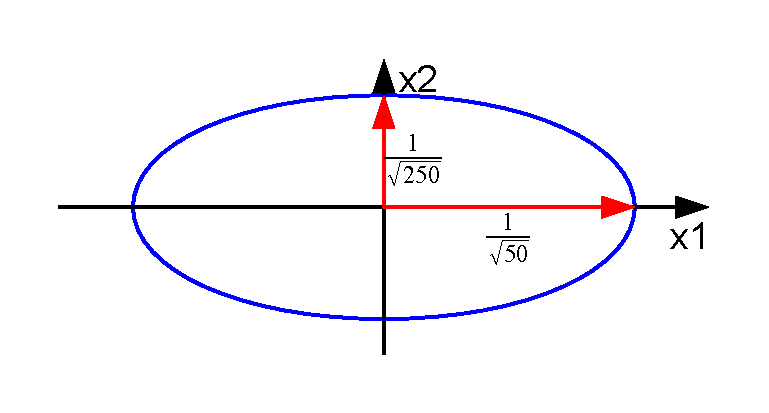
\includegraphics[scale=0.8]{images/quadrik_2d_ellipse_uebung.pdf}\\
	Kommentar zu Grafik: x2,x3 und senkrechte Striche einfügen\\
\end{center}
Bemerkungen: blauer Kreis zeigt den Widerstand, ist dieser Gross leitet es schlecht, ist der Widerstand klein leitet es gut.
\\
\\
b) Transformation $30^\circ$
\begin{align}
k_{ij}'=RkR^{T}
\end{align}

\begin{align}
\phi=+30^\circ
\end{align}

\begin{align}
k_{ij}'=\begin{pmatrix}
\cos{\phi} & -\sin{\phi} & 0 \\
\sin{\phi} & \cos{\phi} & 0 \\
0 & 0 & 1
\end{pmatrix}
\cdot
\begin{pmatrix}
50 & 0 & 0 \\
0 & 250 & 0 \\
0 & 0 & 250 
\end{pmatrix}
\cdot
\begin{pmatrix}
\cos{\phi} & \sin{\phi} & 0 \\
-\sin{\phi} & \cos{\phi} & 0 \\
0 & 0 & 1
\end{pmatrix}
\end{align}

\begin{align}
k_{ij}'=\begin{pmatrix}
100 & -86.60 & 0 \\
-86.60 & 200 & 0 \\
0 & 0 & 250
\end{pmatrix}
\end{align}
\qed

c) Heatflow in x1 Direction, $30^\circ$ Rotated Material

Alle Ableitungen bis auf $\frac{\partial T}{\partial x1}=a$ sind 0


\begin{align}
j_i=-k_{ij} \frac{\partial T}{\partial x_j}
\end{align}

\begin{align}
\vec{j}=\begin{pmatrix}
100 \\
-86.6 \\
0
\end{pmatrix}
\cdot -a
\end{align}

\qed
d) Ellipsoid

\begin{center}
	Gedrehter Tensor (nicht im Hauptachsensystem):\\
	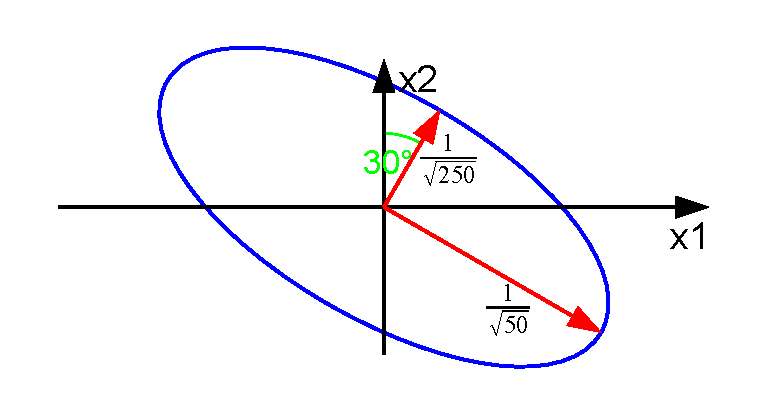
\includegraphics[scale=0.8]{images/quadrik_2d_ellipse_uebung_rotation.pdf}\\
	Kommentar zur Grafik: x2,x3 und schräge Striche einfügen\\
\end{center}

e) Determine the resistivity $r_{12}$

\begin{align}
r_{ij}=\frac{1}{k_{ij}}=\begin{pmatrix}
\frac{1}{k_{11}} & 0 & 0 \\
0 & \frac{1}{k_{22}} & 0 \\
0 & 0 & \frac{1}{k_{33}}
\end{pmatrix}
\end{align}

\begin{align}
r_{ij}'=Rr_{ij}R^{T} = \begin{pmatrix}
16 & 6.9 & 0 \\
6.9 & 8 & 0 \\
0 & 0 & 4
\end{pmatrix}
10^{-3}[\frac{mK}{W}] 
\end{align}
\qed




\subsubsection{Eletrical Tin}
Write down the conductivity Tensor:\\
(Bemerkung: andere Materialwerte sind im Skript, Kapitel 4 auf der Seite 6 zu finden)

\begin{align}
\sigma_{ij} = \frac{1}{\rho_{ij}}= \begin{pmatrix}
101 & 0 & 0 \\
0 & 101 & 0 \\
0 & 0 & 69.9 
\end{pmatrix}
10^5 [\frac{S}{m}]
\end{align}



a) Calculate the magnitude and the direction of the current density

\begin{align}
j_i=\sigma_{ij}E_j
\end{align}

Multiplizieren mit Feld...
\\... z.B. $ j_i=\sigma_{ij}E_j = \sigma_{ij} = \frac{1}{\rho_{ij}}= \begin{pmatrix}
101 & 0 & 0 \\
0 & 101 & 0 \\
0 & 0 & 69.9 
\end{pmatrix} 10^5 [\frac{S}{m}] 
\begin{pmatrix}
0 \\
0.5 \\
0.866 \\
\end{pmatrix} [\frac{V}{m}] = 
\begin{pmatrix}
0 \\
5.05 \\
6.05 \\
\end{pmatrix} 10^5 [\frac{A}{m^2}]$



Danach Vektorbetrag und Winkel berechnen. :-)\\

Vektorbetrag: 

\begin{align}
j_i=\sqrt{j_x^2+j_y^2+j_z^2}
\end{align}
... z.B. $\sqrt{ 0^2+(5.05 \cdot 10^5)^2+(5.05 \cdot 10^5)^2 } = 7.88 [\frac{A}{mm^2}]$ 
\\
\\
Winkel:

\begin{align}
\tan{\alpha}=\frac{Gegenkathete}{Ankathete} \Rightarrow \alpha=arctan(\frac{Gegenkathete}{Ankathete})
\end{align}
... z.B. $ \alpha=arctan(\frac{Gegenkathete}{Ankathete}) = arctan(\frac{6.05 \cdot 10^5}{5.05 \cdot 10^5}) = 50^\circ $


c) Ellipsoid zeichnen



\qed


\subsection{Exercise}
\subsubsection{Useful formulas}

Gradient von $ (\frac{1}{r}) $  with $ r=\sqrt{x^2+y^2+z^2} $

Anwenden von der Produktregel eines Gradient, siehe Formel \ref{eqn:ProduktregelEinesGradientMitPotenzen} auf Seite \pageref{eqn:ProduktregelEinesGradientMitPotenzen}

$ \nabla(\frac{1}{r}) = -\frac{\vec{r}}{r^3}$
\\
$ \nabla(\frac{1}{r^2}) = -2\frac{\vec{r}}{r^4}$
\\
$ \nabla(\frac{1}{r^3}) = -3\frac{\vec{r}}{r^5}$

\subsubsection{The electrical field}

Info A\\
Berechnung von curl von einer Punktladung.\\ 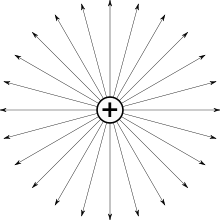
\includegraphics[scale=0.2]{images/punktladung.png}
\label{fig:Punktladung}

$ \vec{E}(\vec{r})=\frac{q}{4\Pi\epsilon_0}\frac{\vec{r}}{r^3}\sim \frac{\vec{r}}{r^3} $
\\
$ \vec{\nabla}\times\vec{E}\approx\vec{\nabla}\times(\frac{\vec{r}}{\vec{r^3}})=\frac{\vec{1}}{r^3}(\vec{\nabla}\times\vec{r})+\vec{r}\times(\vec{\nabla}(\frac{1}{r^3}))=-\frac{3}{r^5}(\vec{r}\times\vec{r})=0 $

Info B\\
$ k=\frac{1}{4\pi\epsilon_0} $

Info C\\


Info D\\

\subsubsection{Polar Molecules (Torque and force)}

torque on molecule by an electrical field\\

$ \vec{F}=q\cdot\vec{E}$\\

$ \vec{M}=\vec{r}\cdot\vec{F}$\\

$ \vec{M}=\vec{p}\times\vec{E}$\\

Non uniform E-Field\\

\begin{align}
\vec F = \begin{pmatrix}
P_x \frac{\partial E_x}{\partial x} + P_y \frac{\partial E_x}{\partial y} + P_z
\frac{\partial E_x}{\partial z}\\
P_x \frac{\partial E_y}{\partial x} + P_y \frac{\partial E_y}{\partial y} + P_z
\frac{\partial E_y}{\partial z}\\
P_x \frac{\partial E_z}{\partial x} + P_y \frac{\partial E_z}{\partial y} + P_z
\frac{\partial E_z}{\partial z}\\
\end{pmatrix}
= \operatorname{grad} (\vec E) \cdot \vec p
\end{align}


\subsection{Elasticity}
\begin{minipage}{3cm}
	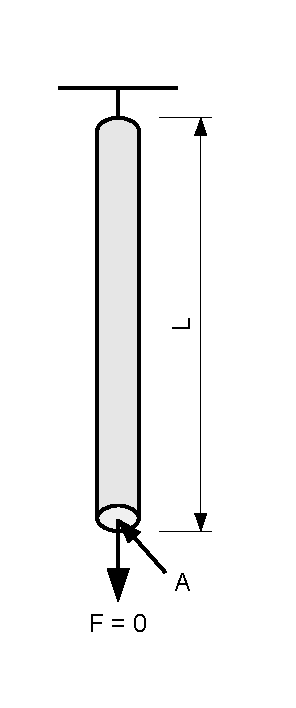
\includegraphics[scale=0.6]{images/elasticity_robe.pdf}
\end{minipage}
\hfill
\begin{minipage}{14cm}
	Balance equation: $0 = \frac{\partial \sigma_{11}}{\partial x} + \rho g_1$\\
	Material law: $\epsilon_{11} = \frac{\partial u(x)}{\partial x}$ with
	$\sigma_{11} = E \cdot \epsilon_{11}$\\
	Boundary conditions: $\sigma_{11} (L) = \frac{F}{A}$, $u(0)= 0$\\
	
	DGL aufstellen: $\frac{\partial \sigma (x)}{\partial x} = - \rho g$ $\mid$ $\int
	dx$\\
	DGL lösen: $\sigma (x) = - \rho g x + \sigma_0$\\
	Boundary Conditions bei L: $\sigma (L) = \frac{F}{A} = \frac{0}{A} = 0$\\
	BC in DGL einsetzen: $\sigma (L) = - \rho g L + \sigma_0 = 0$\\
	Auflösen: $\sigma_0 = \rho g L$\\
	In DGL einsetzen: $\sigma (x) = - \rho g x + \rho g L = \rho g (L-x)$\\
	Material law: $\epsilon (x) = \frac{\rho g}{E} (L-x)$\\
	Aus Material law: $\frac{\partial u(x)}{\partial x} = \epsilon (x) = \frac{\rho
		g}{E} (L-x)$ $\mid$ $\int dx$\\
	Deformation: $u(x) - u(0) = \int\limits_{0}^{x} dx' \cdot \epsilon(x') =
	\int\limits_{0}^{x} \frac{\rho g}{E} (L-x) dx = \frac{\rho g}{E} (x \cdot L -
	\frac{1}{2} \cdot x^2) = \frac{\rho g}{E} \cdot x(L-\frac{x}{2})$, wobei $u(0) =
	0$\\
	Wichtig x' statt x verwenden, u(x) ist gemeint dasss wir die Dehnung von 0 bis
	zu einem Punkt zwischen 0 und L integrieren!\\
	
\end{minipage}
\textbf{Maximaler Stress} tritt an der Aufhängung an Punkt $x = 0$ auf:\\
$\sigma(0) = - \rho g (L-x) = \rho g L = \frac{m \cdot g}{A}$\\
Einheitenkontrolle: $[\rho \cdot g \cdot L] = \frac{kg}{m^3} \cdot
\frac{m}{s^2} \cdot m = \frac{kg}{m \cdot s^2}$\\
$[m \cdot g \cdot \frac{1}{A}] = kg \cdot \frac{m}{s^2} \cdot \frac{1}{m^2} =
\frac{kg}{m \cdot s^2}$\\
\subsubsection{Nochmals das gleiche mit Gewicht}
$F \neq 0$ $\to$ $\sigma(L) = \frac{M
	g}{A}$\\
DGL aufstellen: $\frac{\partial \sigma (x)}{\partial x} = - \rho g$ $\mid$
$\int dx$\\
DGL lösen: $\sigma (x) = - \rho g x + \sigma_0$\\
Boundary Conditions bei L: $\sigma (L) = \frac{F}{A} = \frac{M g}{A}$\\
BC in DGL einsetzen: $\sigma (L) = - \rho g L + \sigma_0 = \frac{M g}{A}$\\
Auflösen: $\sigma_0 = \rho g L + \frac{M
	g}{A}$\\
In DGL einsetzen: $\sigma (x) = - \rho g x + \rho g L + \frac{M g}{A}= \rho g
(L-x) + \frac{M g}{A}$\\
Material law: $\epsilon (x) = \frac{\rho g}{E} (L-x) + \frac{M g}{E A}$\\
Aus Material law: $\frac{\partial u(x)}{\partial x} = \epsilon (x) = \frac{\rho
	g}{E} (L-x) + \frac{M g}{E A} =  \frac{g}{E} (\rho L + \frac{M}{A} - \rho x) $
$\mid$ $\int dx$\\
Deformation: $u(x) - u(0) = \int\limits_{0}^{x} \epsilon(x) dx =
\int\limits_{0}^{x} \frac{g}{E} (\rho L + \frac{M}{A} - \rho x) dx =
\frac{g}{E} \cdot x \left( \left( L \rho + \frac{M}{A} \right) -
\frac{x \rho}{2}\right)$, wobei $u(0) = 0$\\

\subsubsection{Spring Constant (Federkonstante)}
Definition Federkonstante: $F = d \cdot \Delta u $\\
$\sigma = \frac{F}{A}$ $\Rightarrow$ (siehe Übung oben) $u(x) = \frac{F}{A E}
x$\\
Für 1D und isotrop über ganzes Gummiband: $x = L$\\
$\Delta u = \frac{F L}{A E}$\\
Aus $F = d \cdot \Delta u $ ergibt sich: $d = \frac{A E}{L}$

\subsection{Beispiel Teil 2 (Strain, Stress, \ldots)} % Exercises Week 9

\subsubsection{Pure Shear Stress}

\textbf{Momentum flux}\\
\begin{minipage}{6cm}
	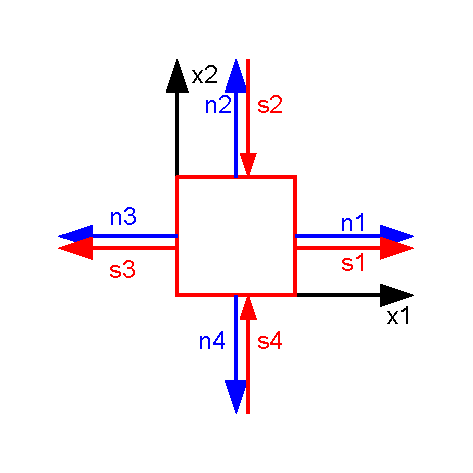
\includegraphics[scale=0.8]{images/pure_shear_stress_1.pdf}
\end{minipage}
\hfill
\begin{minipage}{14cm}
	Gegeben: $\sigma = \begin{pmatrix}
	s & 0 & 0\\
	0 & -s & 0\\
	0 & 0 & 0\\
	\end{pmatrix} $\\
	cutting forces on each face:\\
	$s_1 = \sigma \vec n_1 = \begin{pmatrix}
	s & 0\\
	0 & -s\\
	\end{pmatrix} \begin{pmatrix}
	1\\
	0\\
	\end{pmatrix} = \begin{pmatrix}
	s\\
	0\\
	\end{pmatrix}$\\
	
	$s_2 = \sigma \vec n_2 = \begin{pmatrix}
	s & 0\\
	0 & -s\\
	\end{pmatrix} \begin{pmatrix}
	0\\
	1\\
	\end{pmatrix} = \begin{pmatrix}
	0\\
	-s\\
	\end{pmatrix}$\\
	
	$s_3 = \sigma \vec n_3 = \begin{pmatrix}
	s & 0\\
	0 & -s\\
	\end{pmatrix} \begin{pmatrix}
	-1\\
	0\\
	\end{pmatrix} = \begin{pmatrix}
	-s\\
	0\\
	\end{pmatrix}$\\
	
	$s_4 = \sigma \vec n_4 = \begin{pmatrix}
	s & 0\\
	0 & -s\\
	\end{pmatrix} \begin{pmatrix}
	0\\
	-1\\
	\end{pmatrix} = \begin{pmatrix}
	0\\
	s\\
	\end{pmatrix}$
	
\end{minipage}

\textbf{Transform}\\
Transformation as usual:
\begin{align}
	\sigma'_{kl}=R_{ki}R_{lj}\sigma_{ij}=R_{ki}\sigma_{ij}R_{jl}^T \\
	R_{kl}=\begin{pmatrix} 
		\cos \alpha & -\sin \alpha & 0 \\
		\sin \alpha &  \cos \alpha & 0 \\            
		0        &  0           & 1
	\end{pmatrix}
\end{align}

Resultat:

\begin{align}
	\sigma'_{kl}=\begin{pmatrix}
		0 & s & 0 \\
		s & 0 & 0 \\
		0 & 0 & 0
	\end{pmatrix}
\end{align}

\begin{minipage}{6cm}
	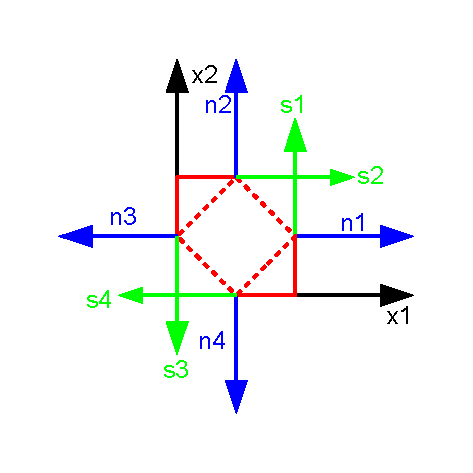
\includegraphics[scale=0.8]{images/pure_shear_stress_2.pdf}
\end{minipage}
\hfill
\begin{minipage}{14cm}
	cutting forces on each face:\\
	$s_1 = \sigma \vec n_1 = \begin{pmatrix}
	0 & s\\
	s & 0\\
	\end{pmatrix} \begin{pmatrix}
	1\\
	0\\
	\end{pmatrix} = \begin{pmatrix}
	0\\
	s\\
	\end{pmatrix}$\\
	
	$s_2 = \sigma \vec n_2 = \begin{pmatrix}
	0 & s\\
	s & 0\\
	\end{pmatrix} \begin{pmatrix}
	0\\
	1\\
	\end{pmatrix} = \begin{pmatrix}
	s\\
	0\\
	\end{pmatrix}$\\
	
	$s_3 = \sigma \vec n_3 = \begin{pmatrix}
	0 & s\\
	s & 0\\
	\end{pmatrix} \begin{pmatrix}
	-1\\
	0\\
	\end{pmatrix} = \begin{pmatrix}
	0\\
	-s\\
	\end{pmatrix}$\\
	
	$s_4 = \sigma \vec n_4 = \begin{pmatrix}
	0 & s\\
	s & 0\\
	\end{pmatrix} \begin{pmatrix}
	0\\
	-1\\
	\end{pmatrix} = \begin{pmatrix}
	-s\\
	0\\
	\end{pmatrix}$\\
	
\end{minipage}

\textbf{Trace}\\

\begin{align}
	\operatorname{tr}\sigma_{kl}=0 \\
	\operatorname{tr}\sigma'_{kl}=0 
\end{align}

$\Rightarrow$ Pure Shear Stress
\qed
\subsubsection{Stress in the Principal Axis System}
Gegeben:
\begin{align}
	\sigma=\begin{pmatrix}
		-\frac{2}{25} & 0 & \frac{36}{25} \\
		0 & 3 & 0 \\
		\frac{36}{25}& 0 & -\frac{23}{25}
	\end{pmatrix}
\end{align}

Find Eigenvalues:

\begin{align}
	\operatorname{eig}(\sigma)=\left(1,-2, 3\right) \operatorname{or}
	\left(1,3,-2\right)
\end{align}
Eigenwerte werden standardmässig nach Grösse geordnet (Reihenfolge jedoch nicht
relevant, ergibt anderes Koordinatensystem).


Resultat:

\begin{align}
	\sigma'=\begin{pmatrix}
		1 & 0 & 0 \\
		0 & 3 & 0 \\
		0 & 0 & -2
	\end{pmatrix}
\end{align}

Aufteilung des Stresstensor siehe Kapitel \ref{stressdecomposition} auf Seite
\pageref{stressdecomposition}!

\subsubsection{Deformation Strain State}\label{9.3} % Exercises Week 9.3
Gegeben Deformation: $u = (a \cdot x_2, b \cdot x_2, 0)^T$

b) Gradient der Deformation: $e_ij= \frac{\partial u_i}{\partial x_j} => e =
\begin{bmatrix}
0 & a & 0\\
0 & b & 0\\
0 & 0 & 0\\
\end{bmatrix}$\\
In symmetrischen und antisymmetrischen Teil splitten: $e = e^{sym} + e^{anti}=
\begin{pmatrix}
0 & a/2 & 0\\
a/2 & b & 0\\
0 & 0 & 0\\
\end{pmatrix}
+
\begin{pmatrix}
0 & a/2 & 0\\
-a/2 & 0 & 0\\
0 & 0 & 0\\
\end{pmatrix}$\\
Symmetrischer Part: $\epsilon = \begin{pmatrix}
0 & a/2 & 0\\
a/2 & b & 0\\
0 & 0 & 0\\
\end{pmatrix}$, da $\epsilon_{33} = \epsilon_{13} = \epsilon_{23}= 0$ $\rightarrow$ plane
strain\\
Antisymmetrischer Part: $\gamma = \begin{pmatrix}
0 & a/2 & 0\\
-a/2 & 0 & 0\\
0 & 0 & 0\\
\end{pmatrix}$ $\rightarrow$ Korrespondiert zu einer Drehung um die z-Achse mit
dem Winkel $\Phi \approx -\frac{a}{2}$ (für kleine Winkel), Drehmatrix:
$R_z(\alpha) = \begin{pmatrix} \cos \alpha & -\sin \alpha & 0 \\
\sin \alpha &  \cos \alpha & 0 \\            
0        &  0           & 1
\end{pmatrix}$

c) Find a deformation vector $u(x)$ reproducing the symmetric part of the strain
tensor that is as symmetric as possible with respectq to $x_1$ and $x_2$. Depict
this new deformation graphically and interpret the relation of the old
deformation, the antisymmetric part in the light of the new deformation.\\

$u(x) = \epsilon \cdot \begin{pmatrix} x_1\\ x_2\\ x_3\\ \end{pmatrix} =
\begin{pmatrix} 0 & a/2 & 0\\
a/2 & b & 0\\
0 & 0 & 0\\
\end{pmatrix} \cdot \begin{pmatrix} x_1\\ x_2\\ x_3\\ \end{pmatrix} =
\begin{pmatrix}
\frac{a}{2} \cdot x_2\\ \frac{a}{2} \cdot x_1 + b \cdot x_2\\ 0\\ \end{pmatrix}$

d) Tensor aufteilen (Volumenerhaltung (volume preserving))\\
$\epsilon =
\underbrace{
	\begin{pmatrix}
	b/3 & 0 & 0\\
	0 & b/3 & 0\\
	0 & 0 & b/3\\
	\end{pmatrix}
}_{\text{Volumenänderung}} +
\underbrace {
	\begin{pmatrix}
	-b/3 & a/2 & 0\\
	a/2 & 2b/3 & 0\\
	0 & 0 & -b/3\\
	\end{pmatrix}}_{\begin{matrix} Spur = 0\\ \text{keine Volumenänderung}\\
	\end{matrix}}$

e) Relative Volumenänderung: $\frac{\Delta V}{V} = \frac{b}{3} + \frac{b}{3} +
\frac{b}{3} = b$

\subsection{Beispiel Elastizität II} % Exercises of Chapter 10

\subsubsection{Elasticity Tensor and Projections} % Aufgabe 10.1
Show that:
\begin{align}\label{eq:10.1a}
	\frac{1}{3} \mathbb{E} : \frac{1}{3} \mathbb{E} = \frac{1}{3}
	\mathbb{E}
\end{align}
Definition E: $E_{ijkl} = \delta_{ij} \delta_{kl}$\\
Formel \ref{eq:10.1a} in Komponenten repräsentation:
\begin{align}
	\frac{1}{9} E_{ijkl} E_{klpq} = \frac{1}{9} \delta_{ij} \delta_{kl} \delta_{kl}
	\delta_{pq} = \frac{1}{9} \delta_{ij} \delta_{kk} \delta_{pq} = \frac{1}{3}
	E_{ijpq}
\end{align}

\subsubsection{E-Modul Along Special Directions} % Aufgabe 10.4

\textbf{E-Modul Silicon along one axis}\\
Determine the E-module for Si in the direction along one of the cubic
axes\\

Spannung in [1, 0, 0] Richtung: $\sigma = (\sigma_{11}, 0, 0, 0, 0, 0)^T$\\

Beziehung gegeben: $\sigma = \mathbb{C} \epsilon$ Umgeformt: $\epsilon =
\mathbb{C}^{-1} \sigma$\\

Für $\mathbb{C}$ gilt (fliegt von SkriptHimmel):
\begin{align}
	\mathbb{C}^{cube} = \begin{pmatrix}
		C_{11} & C_{12} & C_{12} & 0 & 0 & 0\\
		C_{12} & C_{11} & C_{12} & 0 & 0 & 0\\
		C_{12} & C_{12} & C_{11} & 0 & 0 & 0\\
		0 & 0 & 0 & C_{44} & 0 & 0\\
		0 & 0 & 0 & 0 & C_{44} & 0\\
		0 & 0 & 0 & 0 & 0 & C_{44}\\
	\end{pmatrix}
\end{align}
with:
\begin{align}
	\begin{pmatrix}
		C_{11} = 166 GPa\\
		C_{12} = 64 GPa\\
		C_{44} = 79.6 GPa\\
	\end{pmatrix}
\end{align}
Dabei interessiert uns nur der obere Teil:
\begin{align}
	\mathbb{C} = \begin{pmatrix}
		C_{11} & C_{12} & C_{12}\\
		C_{12} & C_{11} & C_{12}\\
		C_{12} & C_{12} & C_{11}
	\end{pmatrix}
\end{align}
Diesen Invertieren:
\begin{align}
	\mathbb{C}^{-1} = \begin{pmatrix}
		\frac{C_{11} + C_{12}}{C_{11}^2 + C_{11} \cdot C_{12} - 2 \cdot C_{12}^2} &
		\frac{-C_{11}}{C_{11}^2 + C_{11} \cdot C_{12} - 2 \cdot C_{12}^2} &
		\frac{-C_{11}}{C_{11}^2 + C_{11} \cdot C_{12} - 2 \cdot C_{12}^2}\\
		\frac{-C_{11}}{C_{11}^2 + C_{11} \cdot C_{12} - 2 \cdot C_{12}^2} &
		\frac{C_{11} + C_{12}}{C_{11}^2 + C_{11} \cdot C_{12} - 2 \cdot C_{12}^2} & 
		\frac{-C_{11}}{C_{11}^2 + C_{11} \cdot C_{12} - 2 \cdot C_{12}^2}\\
		\frac{-C_{11}}{C_{11}^2 + C_{11} \cdot C_{12} - 2 \cdot C_{12}^2} &
		\frac{-C_{11}}{C_{11}^2 + C_{11} \cdot C_{12} - 2 \cdot C_{12}^2} &
		\frac{C_{11} + C_{12}}{C_{11}^2 + C_{11} \cdot C_{12} - 2 \cdot C_{12}^2}
	\end{pmatrix}
\end{align}
Da alles ausser $\sigma_{11}$ gleich 0 ist, gilt:
\begin{align}
	\epsilon_{11} = C_{11} \sigma_{11}
\end{align}
Umgeformt und eingesetzt:
\begin{align}
	E_{[100]} = \frac{\sigma_{11}}{\epsilon_{11}} = \frac{1}{C_{11}} =
	\frac{C_{11}^2 + C_{11} \cdot C_{12} - 2 \cdot C_{12}^2}{C_{11} + C_{12}} = 130
	GPa
\end{align}


\textbf{E-Modul Silicon diagonal face}\\


Spannung in [1, 0, 0] Richtung: $\sigma = (\sigma_{11}, 0, 0, 0, 0, 0)^T$\\

Beziehung gegeben: $\sigma = \mathbb{C} \epsilon$ Umgeformt: $\epsilon =
\mathbb{C}^{-1} \sigma$\\


Stelle $\mathbb{C}$ mit

\begin{align}
	\mathbb{C}^{cube} = \begin{pmatrix}
		C_{11} & C_{12} & C_{12} & 0 & 0 & 0\\
		C_{12} & C_{11} & C_{12} & 0 & 0 & 0\\
		C_{12} & C_{12} & C_{11} & 0 & 0 & 0\\
		0 & 0 & 0 & C_{44} & 0 & 0\\
		0 & 0 & 0 & 0 & C_{44} & 0\\
		0 & 0 & 0 & 0 & 0 & C_{44}\\
	\end{pmatrix}
\end{align}

mit

\begin{align}
	\begin{pmatrix}
		C_{11} = 166 GPa\\
		C_{12} = 64 GPa\\
		C_{44} = 79.6 GPa\\
	\end{pmatrix}
\end{align}

Wechsle $\sigma$ in die Matrixnotation und drehe $\sigma$ um $\frac{\pi}{4}$
$[1,1,0]$

\begin{align}
	\sigma'=R \sigma R^{T}
\end{align}

Wechsle $\sigma$ wieder in Voigt-Notation

\begin{align}
	\sigma'=\begin{pmatrix}
		\frac{\sigma_{11}}{2} \\
		\frac{\sigma_{11}}{2} \\
		0 \\
		0 \\
		0 \\
		\sigma_{11}
	\end{pmatrix}
\end{align}

Wende $\mathbb{C}^{-1} \cdot \sigma'$ an um $\epsilon'$ zu erhalten

\begin{align}
	\epsilon'=\begin{pmatrix}
		0.00276 \cdot \sigma_{11} \\
		0.00276 \cdot \sigma_{11} \\
		-0.00213 \cdot \sigma_{11} \\
		0 \\
		0 \\
		0.01256 \cdot \sigma_{11}
	\end{pmatrix}
\end{align}

Wechsle $\epsilon'$ wieder in Matrix Notation und transformiere es auf um
$\frac{\pi}{4}$ zurück und wechsle wieder in Voigt Notation.

\begin{align}
	\epsilon=R^{T}\epsilon'R \\
	\epsilon=\begin{pmatrix}
		0.0059 \cdot \sigma_{11} \\
		-0.00038 \cdot \sigma_{11} \\
		-0.00213 \cdot \sigma_{11} \\
		0 \\
		0 \\
		0
	\end{pmatrix}
\end{align}

Rechne $E=\frac{\sigma_{11}}{\epsilon_{11}}$

\begin{align}
	E=\frac{\sigma_{11}}{0.0059 \cdot \sigma_{11}} \\
	E=169GPa
\end{align}

\subsection{Beispiel Structural Mechanics} % Übungsprüfung Problem 4

\begin{figure}[h]
	\begin{center}
		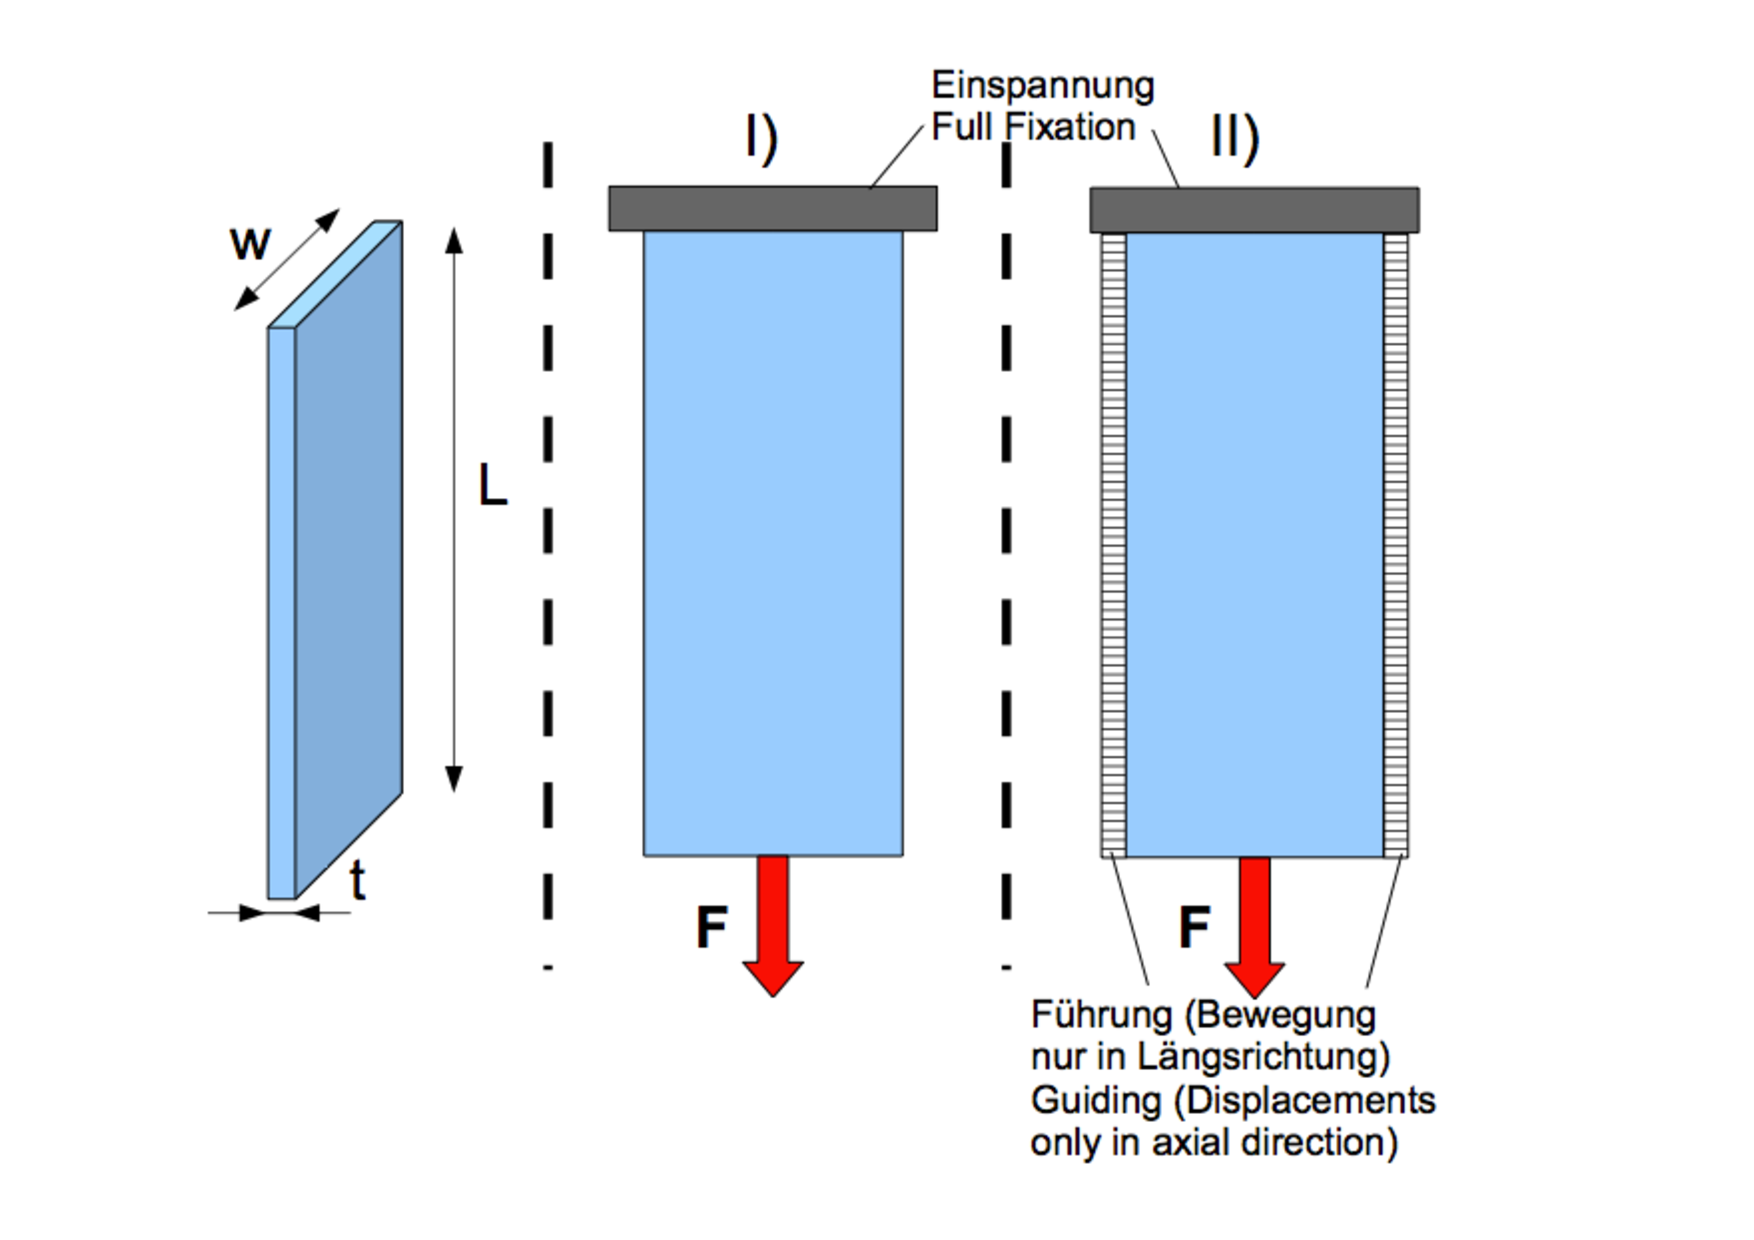
\includegraphics[scale=0.3]{images/structural_mechanics.pdf}
		\caption{Structural Mechanics}
		\label{fig:structuralmechanics}
	\end{center}
\end{figure}

Koordinatensystem: $x_1$: gegen mich, $x_2$: nach rechts, $x_3$ nach unten\\
Länge: $L = 10 cm$, Breite $w=2cm$, Dicke $t=2mm$\\

\textbf{Bestimme die Form des Spannungs- und Verzerrungstensor}\\

\textbf{Fall 1}\\
\begin{align}
	\epsilon_I^{eng} = (-e1, -e_1, e_3, 0, 0, 0)^T
\end{align}
Objekt wird nach unten in die Länge gezogen $e_3$. Dadurch zieht sich
das Objekt in $x_1$ und $x_2$ Richtung zusammen (identisch). Die hinteren
Nullen sind für die Eigenschaften der Scherrung reserviert.\\
\begin{align}
	\sigma_I = (0,0,s_3,0,0,0)^T
\end{align}
Es wirkt nur eine Kraft (Spannung) nach unten.\\

\textbf{Fall 2}\\
\begin{align}
	\epsilon_I^{eng} = (-e1, 0, e_3, 0, 0, 0)^T
\end{align}
Durch die Einspannung kann sich das Objekt in $x_2$ Richtung nicht
zusammenziehen.
\begin{align}
	\sigma_I = (0,s_2,s_3,0,0,0)^T
\end{align}
Daraus folgt, dass die Einspannung als Kraft in $x_2$ Richtung wirken muss.\\

\textbf{Berechnung Verzerrungs- und den Spannungstensor}\\
E-Modul: $E = 70 GPa$, Poissonzahl $\nu = 0.3$\\
Ausgehend von $\sigma = C \cdot \epsilon$:\\
Anhand Formel \ref{eq:elasticity}:
\begin{align}
	\mathbf{C} = \frac{E}{1 + \nu} \cdot \begin{pmatrix}
		\frac{1-\nu}{1-2\nu} & \frac{\nu}{1-2\nu} & \frac{\nu}{1-2\nu}\\
		\frac{\nu}{1-2\nu} & \frac{1-\nu}{1-2\nu} & \frac{\nu}{1-2\nu}\\
		\frac{\nu}{1-2\nu} & \frac{\nu}{1-2\nu} & \frac{1-\nu}{1-2\nu}
	\end{pmatrix}
\end{align}
Ergibt sich:
\begin{align}
	\frac{E}{1 + \nu} \cdot \begin{pmatrix}
		\frac{1-\nu}{1-2\nu} & \frac{\nu}{1-2\nu} & \frac{\nu}{1-2\nu}\\
		\frac{\nu}{1-2\nu} & \frac{1-\nu}{1-2\nu} & \frac{\nu}{1-2\nu}\\
		\frac{\nu}{1-2\nu} & \frac{\nu}{1-2\nu} & \frac{1-\nu}{1-2\nu}
	\end{pmatrix}
	\begin{pmatrix}
		-e_1\\ -e_1\\ e_3
	\end{pmatrix}
	=
	\begin{pmatrix}
		0\\ 0\\ s_3
	\end{pmatrix}
\end{align}
Linie 1 und 2 ergeben identische Formel, wobei Faktoren mit $C_{ij}$
geschrieben werden:
\begin{align}
	(C_{11} + C_{12}) \cdot (-e_1) + C_{12} \cdot e_3 = 0
\end{align}
2te Gleichung, Beachte $\frac{E}{1+\nu}$ ist wohl in den $C_{ij}$ versteckt:
\begin{align}
	2 \cdot C_{11} \cdot (-e_1) + C_{C_12} e_3 = s_3
\end{align}
Bei der Auflösung des Gleichungssystem wird dass Prinzip der Mut zur Lücke laut
der Formel 379 nach Dr. D. Strebel angewahnt!
	\section{Anhang}
	%	
\subsection{Differential-Rechnung}
$f'(x_0)=\lim\limits_{\Delta x\rightarrow 0}
\frac{f(x_0+\Delta)x-f(x_0)}{\Delta x}$\\
\begin{tabular}{llll}
	Kettenregel:	& $f\big(g(x)\big)$ &$=$ & $g'(x)\cdot f'\big(g(x)\big)$
	oder $\frac{d f(g(x))}{dx} = f'(g(x)) \cdot g'(x)$\\[0.1cm] Produktregel:	&
	$f(x)\cdot g(x)$ &$=$ & $f'(x)\cdot g(x) + f(x)\cdot g'(x)$\\[0.1cm] Quotientenregel:& $\frac{f(x)}{g(x)}$ &$=$ & $\frac{f'(x)g(x)-f(x)g'(x)}{g^2(x)}$\\
\end{tabular}


\subsection{Taylor Polynom}
$f(x_0+h)=f(x_0) + f'(x_0)h + \frac{f''(x_0)}{2}h^2 + \frac{f'''(x_0)}{3!}h^3 + \ldots + \frac{f^{(n)}(x_0)}{n!}h^n + R_n(x_0, h)$


\subsection{Integraltable}
\begin{center}	
	\begin{multicols}{2}
		
		\begin{equation}
			\int x^n \dx = \frac{1}{n+1}x^{n+1}, \hspace{1ex} n\neq-1
		\end{equation}
		
		\begin{equation}
			\int \frac{1}{x}\dx = \ln |x|
		\end{equation}
		
		\begin{equation}
			\int u \hspace{2pt} \dd{v} = uv - \int v du
		\end{equation}
		
		
		
		\begin{equation}
			\int e^x \dx = e^x 
		\end{equation}
		
		\begin{equation}
			\int a^x \dx = \frac{1}{\ln a} a^x
		\end{equation}
		
		\begin{equation}
			\int \ln x \dx = x \ln x - x
		\end{equation}
		
		
		\begin{equation}
			\int \sin x \dx = -\cos x
		\end{equation}
		
		\begin{equation}
			\int \cos x \dx = \sin x
		\end{equation}
		
		\begin{equation}
			\int \tan x \dx = \ln |\sec x| 
		\end{equation}
		
		\begin{equation}
			\int \sec x \dx = \ln |\sec x + \tan x|
		\end{equation}
		
		\begin{equation}
			\int \sec^2 x \dx = \tan x
		\end{equation}
		
		\begin{equation}
			\int \sec x \tan x \dx = \sec x
		\end{equation}
		
		\begin{equation}
			\int \frac{a}{a^2+x^2}\dx = \tan^{-1}\frac{x}{a}
		\end{equation}
		
		\begin{equation}
			\int \frac{a}{a^2-x^2}\dx = \frac{1}{2}\ln\left|\frac{x+a}{x-a}\right|
		\end{equation}
		
		\begin{equation}
			\int \frac{1}{\sqrt{a^2-x^2}} \dx = \sin^{-1} \frac{x}{a}
		\end{equation}
		
		\begin{equation}
			\int \frac{a}{x \sqrt{x^2-a^2}} \dx = \sec^{-1} \frac{x}{a}
		\end{equation}
		
		\begin{align}
			\int \frac{1}{\sqrt{x^2-a^2}} \dx &= \cosh^{-1} \frac{x}{a} \\&= \nonumber \ln (x+\sqrt{x^2-a^2})
		\end{align}
		
		\begin{align}
			\int \frac{1}{\sqrt{x^2+a^2}} \dx &= \sinh^{-1} \frac{x}{a} \\&=\nonumber \ln (x+\sqrt{x^2+a^2})
		\end{align}
		
	\end{multicols}
\end{center}		











\end{document}


